%% Copernicus Publications Manuscript Preparation Template for LaTeX Submissions
%% ---------------------------------
%% This template should be used for copernicus.cls
%% The class file and some style files are bundled in the Copernicus Latex Package, which can be downloaded from the different journal webpages.
%% For further assistance please contact Copernicus Publications at: production@copernicus.org
%% https://publications.copernicus.org/for_authors/manuscript_preparation.html


%% Please use the following documentclass and journal abbreviations for preprints and final revised papers.

%% 2-column papers and preprints
\documentclass[journal abbreviation, manuscript]{copernicus}



%% Journal abbreviations (please use the same for preprints and final revised papers)


% Advances in Geosciences (adgeo)
% Advances in Radio Science (ars)
% Advances in Science and Research (asr)
% Advances in Statistical Climatology, Meteorology and Oceanography (ascmo)
% Aerosol Research (ar)
% Annales Geophysicae (angeo)
% Archives Animal Breeding (aab)
% Atmospheric Chemistry and Physics (acp)
% Atmospheric Measurement Techniques (amt)
% Biogeosciences (bg)
% Climate of the Past (cp)
% DEUQUA Special Publications (deuquasp)
% Earth Surface Dynamics (esurf)
% Earth System Dynamics (esd)
% Earth System Science Data (essd)
% E&G Quaternary Science Journal (egqsj)
% EGUsphere (egusphere) | This is only for EGUsphere preprints submitted without relation to an EGU journal.
% European Journal of Mineralogy (ejm)
% Fossil Record (fr)
% Geochronology (gchron)
% Geographica Helvetica (gh)
% Geoscience Communication (gc)
% Geoscientific Instrumentation, Methods and Data Systems (gi)
% Geoscientific Model Development (gmd)
% History of Geo- and Space Sciences (hgss)
% Hydrology and Earth System Sciences (hess)
% Journal of Bone and Joint Infection (jbji)
% Journal of Micropalaeontology (jm)
% Journal of Sensors and Sensor Systems (jsss)
% Magnetic Resonance (mr)
% Mechanical Sciences (ms)
% Natural Hazards and Earth System Sciences (nhess)
% Nonlinear Processes in Geophysics (npg)
% Ocean Science (os)
% Polarforschung - Journal of the German Society for Polar Research (polf)
% Primate Biology (pb)
% Proceedings of the International Association of Hydrological Sciences (piahs)
% Safety of Nuclear Waste Disposal (sand)
% Scientific Drilling (sd)
% SOIL (soil)
% Solid Earth (se)
% State of the Planet (sp)
% The Cryosphere (tc)
% Weather and Climate Dynamics (wcd)
% Web Ecology (we)
% Wind Energy Science (wes)


%% \usepackage commands included in the copernicus.cls:
%\usepackage[german, english]{babel}
%\usepackage{tabularx}
%\usepackage{cancel}
%\usepackage{multirow}
%\usepackage{supertabular}
%\usepackage{algorithmic}
%\usepackage{algorithm}
%\usepackage{amsthm}
%\usepackage{float}
%\usepackage{subfig}
%\usepackage{rotating}

\usepackage{booktabs} 
\usepackage{adjustbox}
\usepackage{longtable}

\begin{document}

\title{Urban Ozone Trends in Europe and the USA (2000-2021)}

% \Author[affil]{given_name}{surname}

\Author[1,2,*][beth.nelson@york.ac.uk]{Beth S.}{Nelson} %% correspondence author
\Author[1,2,*][will.drysdale@york.ac.uk]{Will S.}{Drysdale}

\affil[1]{Wolfson Atmospheric Chemistry Laboratories, Department of Chemistry, University of York, Heslington, York, YO10 5DD, UK}
\affil[2]{National Centre for Atmospheric Science, University of York, York, UK}
\affil[*]{These authors contributed equally to this work.}
%% The [] brackets identify the author with the corresponding affiliation. 1, 2, 3, etc. should be inserted.

%% If an author is deceased, please mark the respective author name(s) with a dagger, e.g. "\Author[2,$\dag$]{Anton}{Smith}", and add a further "\affil[$\dag$]{deceased, 1 July 2019}".

%% If authors contributed equally, please mark the respective author names with an asterisk, e.g. "\Author[2,*]{Anton}{Smith}" and "\Author[3,*]{Bradley}{Miller}" and add a further affiliation: "\affil[*]{These authors contributed equally to this work.}".


\runningtitle{TEXT}

\runningauthor{TEXT}

\received{}
\pubdiscuss{} %% only important for two-stage journals
\revised{}
\accepted{}
\published{}

%% These dates will be inserted by Copernicus Publications during the typesetting process.


\firstpage{1}

\maketitle



\begin{abstract}
Trends in urban O\textsubscript{3} and NO\textsubscript{2} across Europe and the United States of America were explored between 2000-2021. Using surface monitoring site data from the TOAR-II and European Environment Agency databases, piecewise quantile regression (PQR) analysis was performed on 228 O\textsubscript{3} time series (144 European, 84 USA) and 322 NO\textsubscript{2} times series (245 European, 77 USA). The PQR analysis permitted 2 break points over the 23 year period to balance the intent to describe changes over a large time period, while still capturing the abrupt changes that can occur in urban atmospheres. Regressions were performed over quantiles ranging from 0.05 to 0.95 and indications of a slowing in the increase of high European O\textsubscript{3} levels was observed. In Europe, more trends were found to having an increasing O\textsubscript{3} trend between 2015-2021 compared with 2000-2004. The reverse was true in the USA, with a reduction in the number of sites with increasing O\textsubscript{3} trends when the same periods were compared. An analysis of the change points revealed a large proportion of sites in Europe, were the second change point in NO\textsubscript{2} switched from a positive to negative trend, occurred in 2020 (41/43 second change points in this year). This was attributed a reduction in NO\textsubscript{2} due to the COVID-19 pandemic, however, in some cases these increasing trends have sustained beyond the recovery from restrictions. 
\end{abstract}

\section{Introduction}  %% \introduction[modified heading if necessary]
Tropospheric ozone (O\textsubscript{3}) is a greenhouse gas and air pollutant harmful to human health, and plant growth \citep{fleming_2018, mills_2018, szopa_2021}. It is a secondary air pollutant, formed from the photochemical reactions of primary pollutants NO\textsubscript{x} (NO + NO\textsubscript{2}) and volatile organic compounds (VOCs). The chemistry of O\textsubscript{3} formation is non-linear and the effect of changing precursor concentrations can cause O\textsubscript{3} concentrations to increase or decrease depending on the photochemical regime found at a given location \citep{ https://doi.org/10.1029/JD095iD02p01837, SILLMAN2002339}. Despite global successes in reducing primary pollutant emissions over the past few decades, global exposure to O\textsubscript{3} has been increasing throughout the 21st century. This is particularly observed in urban areas, where the vast majority of the global population live, projected to increase to 68\% in 2050 from 55\% in 2018 \citep{un_2019}. In a study of 12946 cities located worldwide, the average mean weighted O\textsubscript{3} concentration increased by 11\% between 2000 and 2019, and the number of cities exceeding the WHO peak season O\textsubscript{3} standard increased from 89\% to 96\% \citep{Malashock_2022}.

Due to the complexity of O\textsubscript{3} production, its trend direction, magnitude, and significance varies by location. A previous study calculated trends in two O\textsubscript{3} metrics globally over the period of 2000 - 2014: 4th highest daily maximum 8-hour O\textsubscript{3} (4MDA8), and the number of days with MDA8 > 70 ppb O\textsubscript{3} (NDGT70) \citep{fleming_2018}. The study used data from 4801 global monitoring sites over this time period. For both of these metrics, downward trends were observed for most of the USA, and some sites in Europe. However, over the period of 2010-2014 (2,600 sites utilised), sites located in regions with the highest O\textsubscript{3} precursor emissions across North America, Europe and East Asia had the highest values in 4MDA8 and NDGT70. In North America and Europe, this was particularly true for California and parts of southern Europe \citep{fleming_2018}.

Since the 1990s, a general downward trend in urban O\textsubscript{3} pollution has been observed in the United States \citep{acp-20-3191-2020}. This reducing trend has been linked to stricter limiting regulations on the emissions of primary pollutants such as NO\textsubscript{x} and VOCs. Although NO\textsubscript{x} and VOC emissions in Europe have also been declining since the late 1980s, the trend in O\textsubscript{3} is less clear due to large inner-annual variation, driven by climate variability and the dispersion and transport of pollutants from other regions \citep{acp-6-51-2006, acp-18-5589-2018}. Between 1995 and 2014, negative trends in the highest O\textsubscript{3} levels across urban sites in Europe were identified due to pollutant emission restrictions across Europe. However, increasing background levels, particularly in northern and eastern Europe, make it difficult to identify strong trends in urban O\textsubscript{3} when transboundary effects are considered \citep{acp-18-5589-2018}. Despite this, a study of 93 suburban and urban sites across Europe identified notable enhancements in O\textsubscript{3} seasonal and annual means between 1995 - 2012, even with the continuous downward trend in anthropogenic emissions across the continent \citep{acp-18-5589-2018}.

Since these earlier studies, much of the literature focuses on the impact of the COVID-19 pandemic on air pollutant concentrations and trends \citep{acp-20-15743-2020, doi:10.1126/sciadv.abd6696, acp-21-4169-2021, SOKHI2021106818}. A study of eleven cities across the world, all of which implemented stringent lockdown measures in early 2020, captured sudden decreases in deweathered NO\textsubscript{2} concentrations, concurrent with sudden increases in O\textsubscript{3}, in most locations \citep{doi:10.1126/sciadv.abd6696}. Another study employing machine learning models to predict business-as-usual levels of pollutants, estimated that NO\textsubscript{2} concentrations were 32\% lower than expected across 102 European urban background locations, whereas O\textsubscript{3} was 21\% higher \citep{acp-21-4169-2021}. It is highly likely that this global event has resulted in perturbations of both long-term NO\textsubscript{2} and O\textsubscript{3} trends, particularly in locations where lockdowns were stringent or lengthy.

This study examines the trends in urban O\textsubscript{3} and NO\textsubscript{2} using monitoring site data from 2020 - 2023. It employs quantile regression and change point detection to construct trends that capture the broad structure of a complex time series, while remaining explainable with concise statistics. Section \ref{sect:method} details the method used to create the trends, section \ref{sect:overview_of_trends} provides a high-level overview of the trends with section \ref{sect:significance_of_trends} focusing on the significance of the trends and highlighting features that are discussed in detail later on. Section \ref{sect:trends_across_quantiles} explores the information that can be gained from trends calculated over a range of quantiles and finally section \ref{sect:case_studies} provides details on some of the features revealed earlier in the analysis. 

\section{Methodology} \label{sect:method}
Hourly NO\textsubscript{2} and O\textsubscript{3} data were obtained for urban sites in the USA and Europe using the TOAR-II \citep{toar_db} and European Environment Agency (EEA) \citep{eea_1, eea_2} databases, using the r-packages toarR \citep{drysdale_2024_14537446} and saqgetr \citep{saqgetr} respectively. Those obtained from the EEA are categorised as urban traffic, urban background and urban industrial, while those from the TOAR database are categorised as urban and suburban. A full list of sites can be found in the supplementary information (table S1).  TOAR-II data was retrieved between 2000-01-01 and 2021-12-31 (the latest available) \textcolor{red}{and EEA data between 2000-01-01 and 2023-12-31, the latter being extended longer so the effects of the COVID-19 pandemic could be observed more clearly.} Time series were quality controlled via threshold, persistence and variance checks similar to those in \textcolor{red}{Wang et al., 2024 - or reference within}: O\textsubscript{3} concentrations were required be between 0 and 500 ppbv, periods where an identical value was repeated 8 or more times in a row were removed as were days where the difference between the minimum and maximum concentration was $\leq$ 2 ppbv. 

After quality control, time series were required to have 80 \% data coverage between 2000-01-01 and 2021-12-31 and for the calculation of annual metrics each individual year was retained if it had more than 60 \% coverage. Additionally, a small number of time series were removed following visual inspection - these are listed in table S2. This resulted in 360 O\textsubscript{3} time series (208 Europe, 152 USA). Trends were calculated on daily averaged data, either the mean or maximum daily 8-hour average (MDA8). For the daily data, subgroups of day (hours between 0800 - 1900 L inclusive) and night (hours between 2000 - 0700 L inclusive) were created, then the daily / MDA8 averages taken. It is common to remove the seasonal component of an ozone time series to improve the accuracy of trends \citep{cooper_2020} and here we subtract monthly mean climatologies for each time series resulting ozone anomalies. 

Trends were estimated for these daily, daily (daytime), daily (nighttime) and MDA8 series in three cases: all data, warm season (April - September) and cold season (October - March). These were calculated following the methodology in and using code provided by  \cite{chang2023guidancenotebeststatistical}. QR calculates a linear model that seeks to minimise the residuals with a defined proportion ($\tau$) of the points above and below the fit line. For example, the scenario $\tau$ = 0.5 splits the data 50:50 above and below the line. QR has the advantage of being insensitive to outliers and the $\tau$ = 0.5 case can be considered analogous to a “median” trend line. This is desirable for the longer-term trends being investigated here. The 1-sigma uncertainly for the QRs were calculated via a moving block bootstrapping method, where the data are subdivided into overlapping blocks that are $n^{1/4}$ points wide (or \textasciitilde{20} points for 20 years of hourly data). These blocks are shuffled to generate a new time series, and replicated 1000 times, and the standard deviation of these replicates calculated. This uncertainty was subsequently used in the determination of the p-value, providing a metric for the significance of the trends. 

Quantile regressions were calculated piecewise with 0 - 2 breakpoints to allow the trends to capture large non-linearities. As urban concentration trends can change sharply (e.g. with policy intervention), this gives the model the freedom to represent these. Limiting the model to a maximum of two breakpoints strikes a balance between capturing sufficiently large-scale changes while still being able to describe a \textasciitilde{20} year time series with a small number of coefficients.

To determine what break points to use on each time series, a range of candidate models were constructed, each with zero, one or two break points. These break points were restricted to be unable to occur within the first or last two years of the time series, nor could they occur within 5 years of each other. They were arbitrarily set to occur on the 1st January in a given year, which was deemed an appropriate degree of freedom given the 20 year span of the time series and locating the break points sub annually does not have a large effect on the resulting trends. For a time series that fully spanned the range of 2000-01-01 - 2021-12-31, 110 models would be created - one with zero break points, 18 with one break point, and 91 with 2. All regressions were calculated at $\tau$ = 0.05, 0.10, 0.25, 0.50, 0.75, 0.95 and 0.95.

To select 'change points' from the array of break points available, the model performance was evaluated via Akaike information criterion (AIC). AIC was chosen as the evaluation criteria oweing to its penalty term penalising models with more break points that do not appreciably improve the model fit over the simpler case, The model with the minimum AIC was selected from the candidate pool as the best fit for a time series at a given $\tau$. Figure \ref{fig:method_plot} demonstrates this process on a single time series. 

\begin{figure}[p]
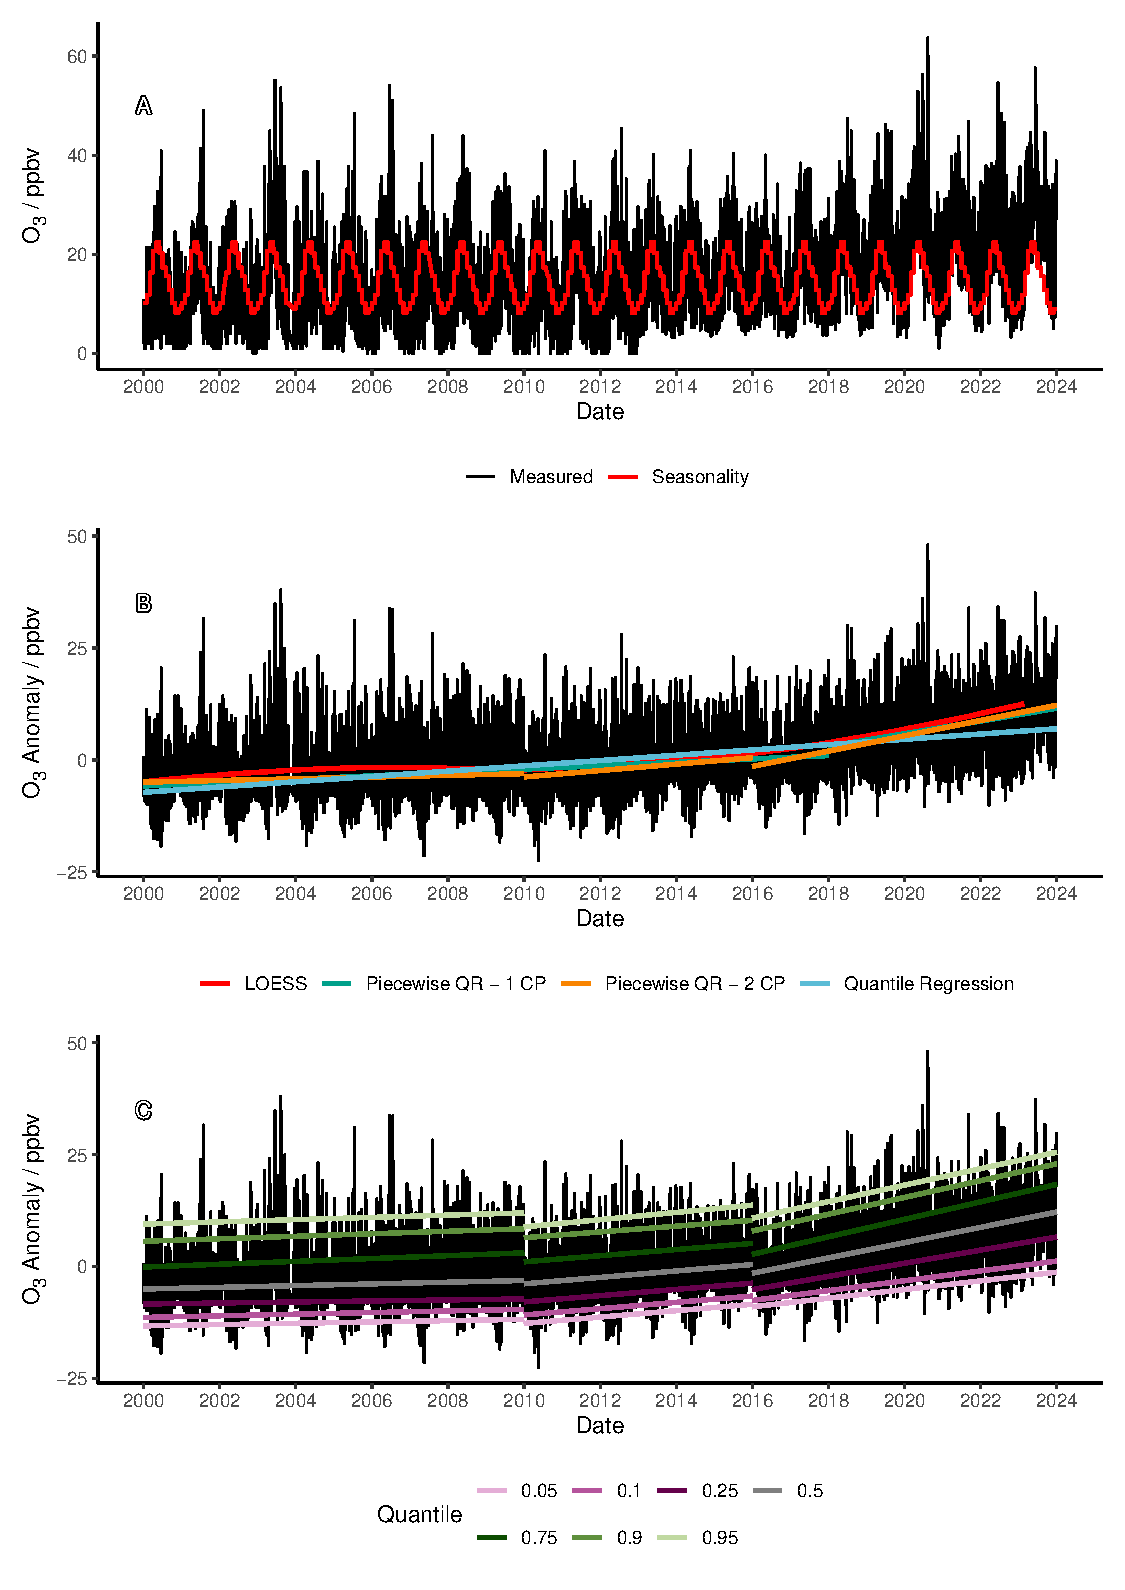
\includegraphics[width=12cm]{figures/f1_method.pdf}
\caption{Example trend determination for an O\textsubscript{3} time series (London Bloomsbury - \textit{GB0566A}). A - O\textsubscript{3} concentration time series (black) and monthly median climatology (red). B - Anomaly time series (black, concentration minus climatology) and 4 trend options, LOESS (red), QR (blue), PQR1 (green) and PQR2 (yellow). C - Anomaly time series (black) and PQR2 across $\tau$ = 0.05, 0.10, 0.25, 0.50, 0.75, 0.90, 0.95. (purple to green)}
\label{fig:method_plot}
\end{figure}


\clearpage
\section{Results and Discussion}

\begin{figure*}[t]
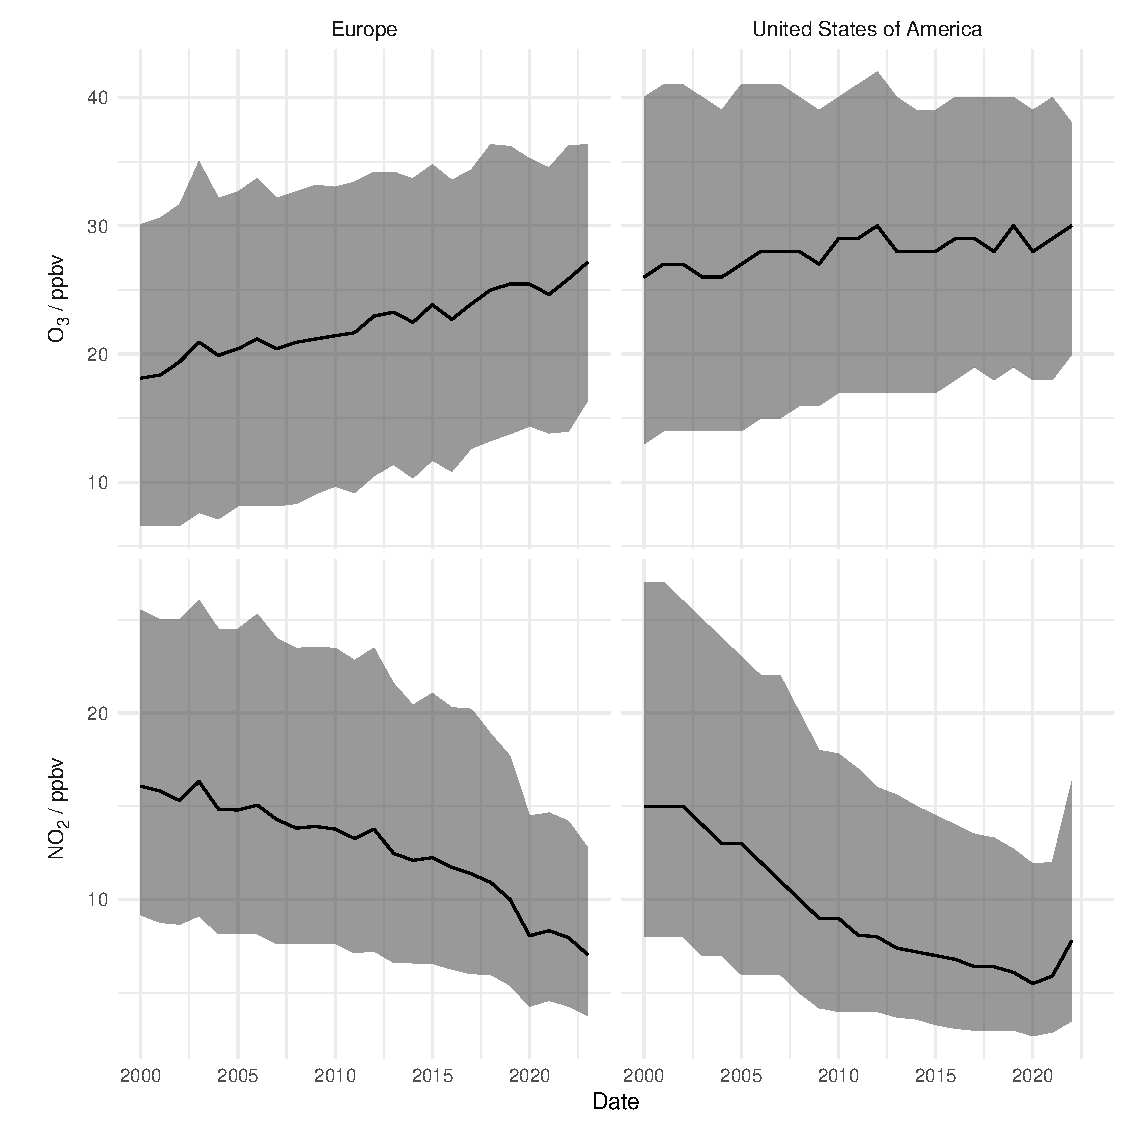
\includegraphics[width=12cm]{figures/f2_conc.pdf}
\caption{Median concentrations of O\textsubscript{3} (top) and NO\textsubscript{2} (bottom) across all sites in this study, separated into sites in Europe (left) and sites in the USA (right).  Shaded regions represent the 25\textsuperscript{th} and 75\textsuperscript{th} percentiles.}
\label{fig:conc_plot}
\end{figure*}

To provide context for the subsequently calculated trends, figure \ref{fig:conc_plot} shows the annual median, 25 th and 75 th percentile concentrations of O\textsubscript{3} and NO\textsubscript{2} across all the urban sites used in this study. Europe shows median O\textsubscript{3} concentrations increasing from 18 ppb to 26 ppb between 2000 and 2019, and USA concentrations increasing, from 26 ppb in 2000 to 30 ppb in 2019. Both Europe and the USA show decreasing NO\textsubscript{2} over the same period (16 ppb to 10 ppb in Europe, 15 ppb to 6 ppb in the USA). The USA does see a return to increasing NO\textsubscript{2} concentrations after 2020, reaching 7.8 ppb in 2022. In section \ref{sect:case_studies} evidence for this increase is discussed. 

%To assess the magnitude of the changing O\textsubscript{3} pollution problem across the USA and Europe, the daily maximum 8-hour running mean for O\textsubscript{3} (MDA8) was calculated. MDA8 is an important metric, used to evaluate whether a particular location is in compliance with, or exceeding, internationally recognised health limits. Air quality guidelines outlined by the World Health Organisation, stipulate a MDA8 limit of 50 ppb (WHO 2005).

The dataset that results from the application of the method described in section \ref{sect:method} has several degrees of freedom to bear in mind during discussion. For a given time series (one species at one site) there are two break points that are common for all the trend lines, and as there are 7 quantiles, this results in 21 slopes, each with an associated p-value. When comparing between sites (or even species within a site) the change points can differ. This is necessary to capture the changing trends observed at urban sites but does complicate describing them. For this discussion we have grouped the sites into those from Europe and those from the United States, though details on individual European countries are available in table S1. 
To aid in summarising, in some cases the results have been grouped into time periods of a few years – in these cases if a trend changes due to a change point both trends have been counted. For example, if between 2000 and 2004 a site were to go from increasing O\textsubscript{3} to decreasing O\textsubscript{3}, this would be described as ‘between 2000 and 2004 there was one increasing O\textsubscript{3} trend and one decreasing O\textsubscript{3} trend’. In the case where a site had a change point in 2003, but the trend remained increasing, this will be counted as one increasing trend. This has the benefit that no one category can count more than then number of available time series. In visualisation, both trends would be shown.

Trends have been collated into significance categories: p $\le$ 0.05 (high certainty), 0.05 $<$ p $\le$ 0.10 (medium certainty), 0.10 $<$ p $\le$ 0.33 (low certainty) and p > 0.33 (very low certainty or no evidence) based off of the guidance of \cite{chang2023guidancenotebeststatistical}. For the most part slopes where the p-value is > 0.33 are treated as ‘no trend’ regardless of their magnitude (generally we observe that as the magnitude of the trend decreases so does its significance), though sometimes are given with a direction when required by a visualisation.

\subsection{Overview of Trends} \label{sect:overview_of_trends}
\begin{figure*}[p]
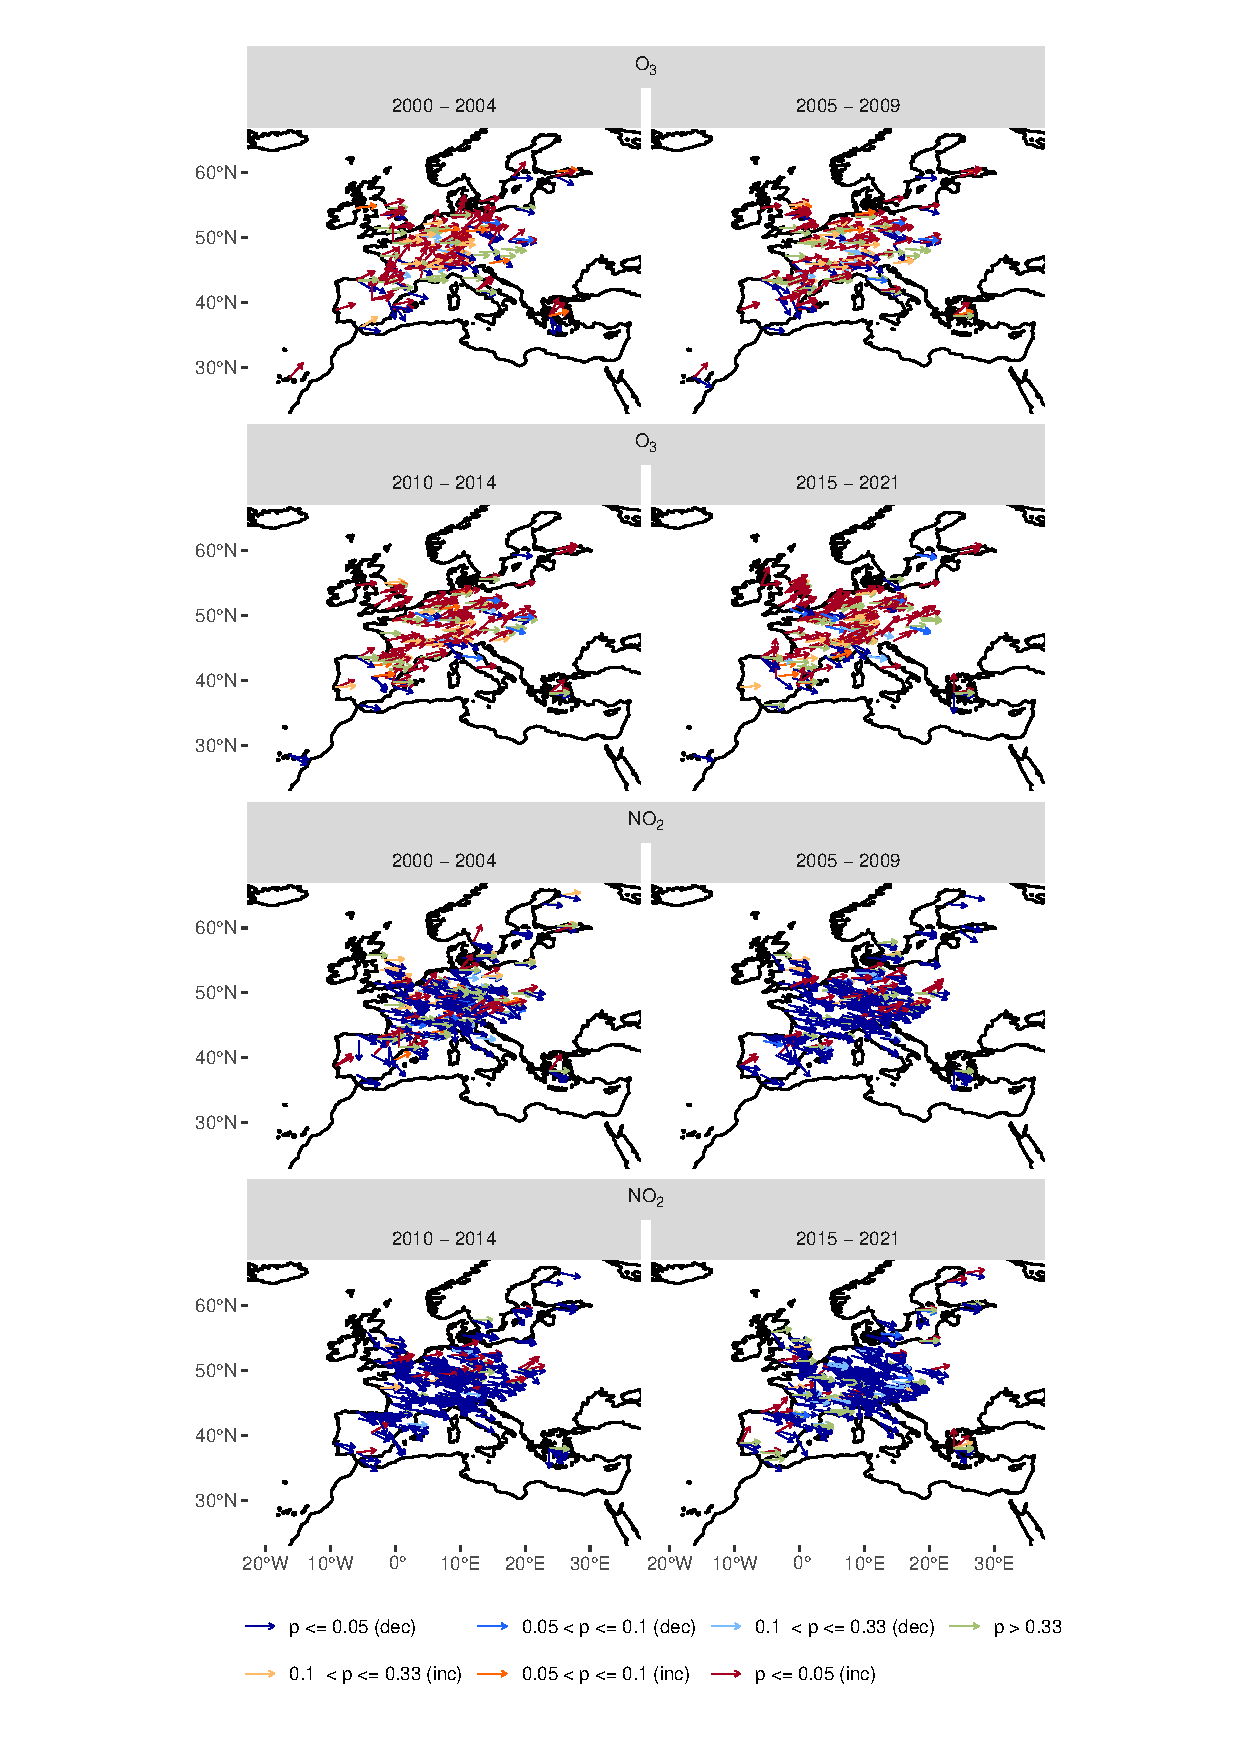
\includegraphics[width=12cm]{figures/f3_eu_arrows.pdf}
\caption{Summary of trends across Europe. Angle of arrow indicates magnitude and direction, with the following orientations: vertical up - +2.5 ppb yr\textsuperscript{-1}, horizontal - 0 ppb yr\textsuperscript{-1} and vertically down - -2.5 ppb yr\textsuperscript{-1}. The few sites with absolute trends > 2.5 ppb yr\textsuperscript{-1} have been clamped to $\pm$ 2.5 ppb yr\textsuperscript{-1}. Colour indicates significance and direction, darkest colours being most significant (p < 0.05) and green the least (p > 0.33). Blues are decreasing trends and reds are increasing trends. The upper 4 plots show O\textsubscript{3} trends, and the lower 4 show NO\textsubscript{2} trends. Each group of 4 groups the trends into segments of the study period. If a change point occurs in a group an arrow for both trends is shown.}

\label{fig:arrow_eu}
\end{figure*}

\begin{figure*}[p]
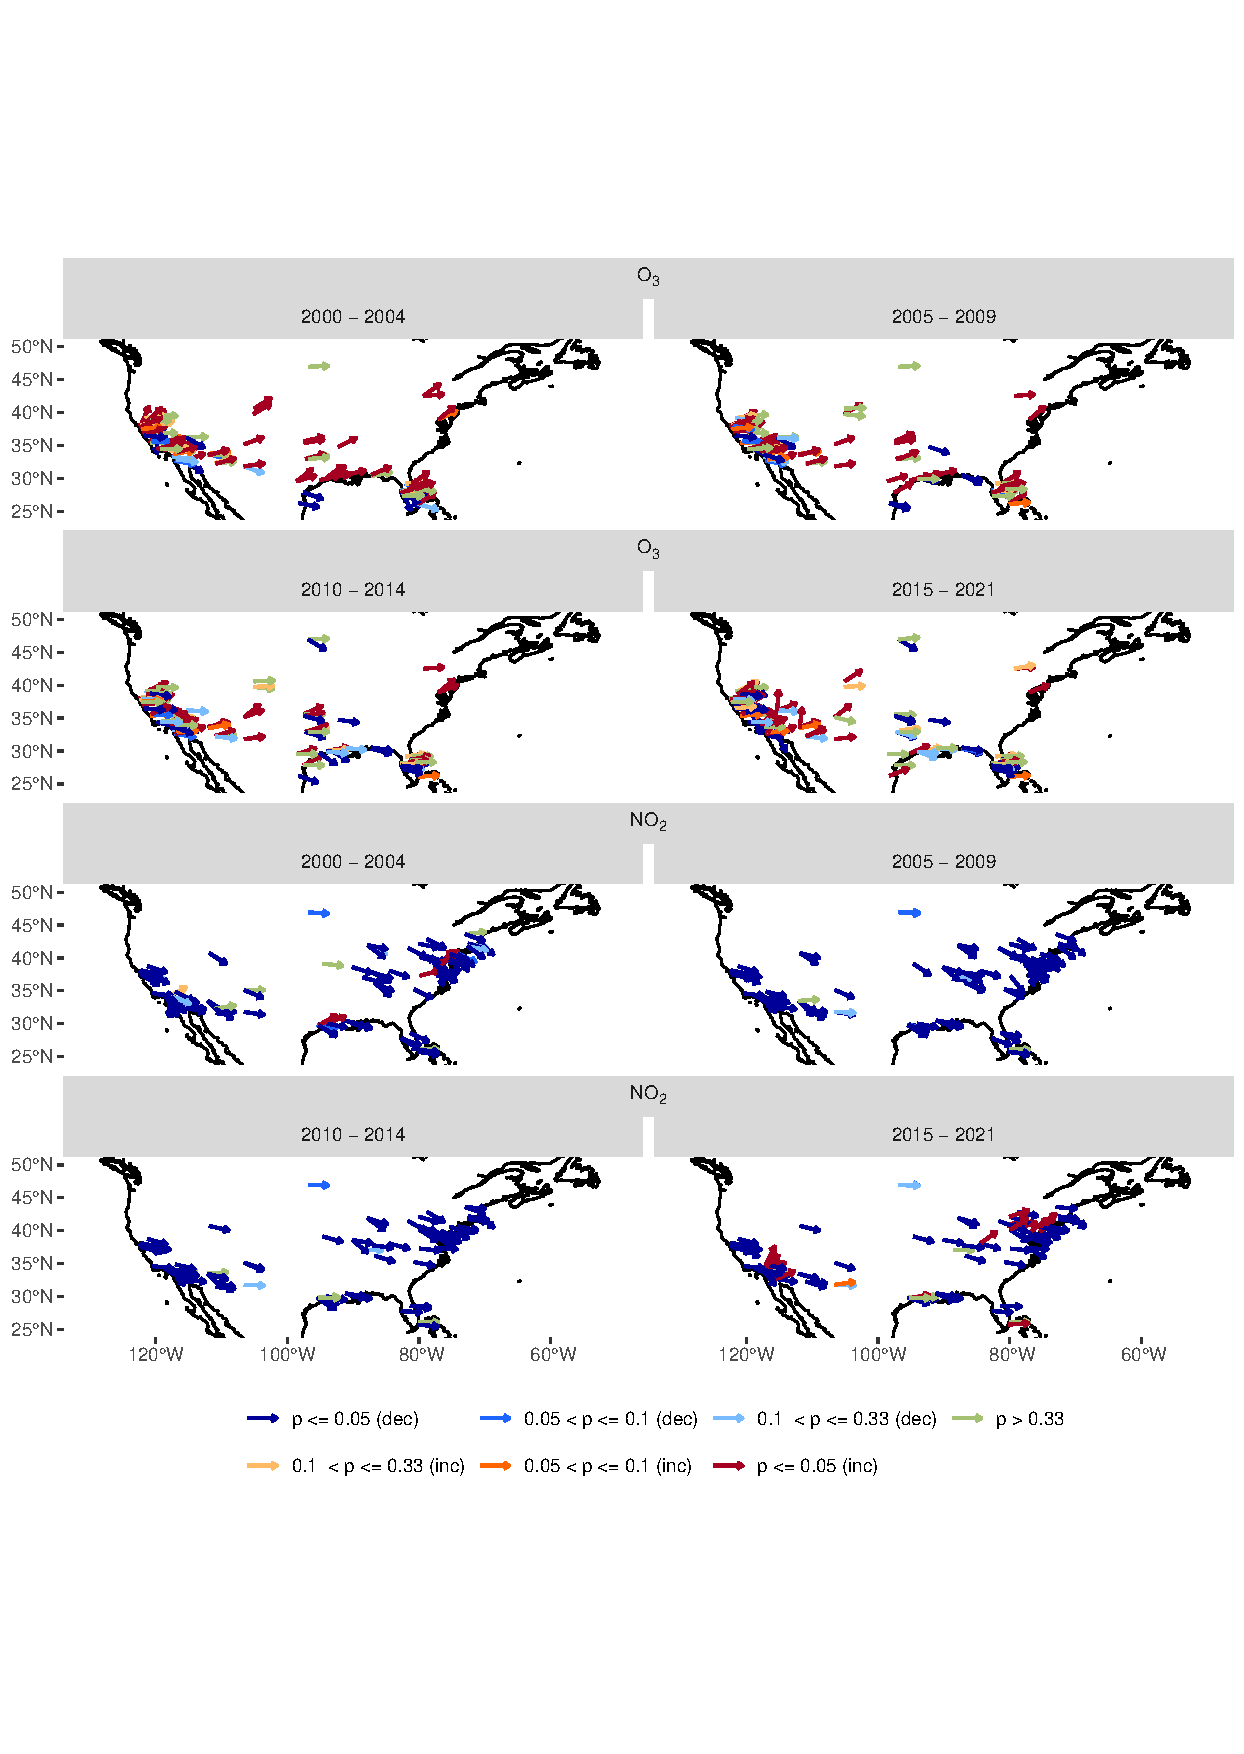
\includegraphics[width=12cm]{figures/f4_usa_arrows.pdf}
\caption{Summary of trends across the United States of America. Angle of arrow indicates magnitude and direction, with the following orientations: vertical up - +2.5 ppb yr\textsuperscript{-1}, horizontal - 0 ppb yr\textsuperscript{-1} and vertically down - -2.5 ppb yr\textsuperscript{-1}. The few sites with absolute trends > 2.5 ppb yr\textsuperscript{-1} have been clamped to $\pm$ 2.5 ppb yr\textsuperscript{-1}. Colour indicates significance and direction, darkest colours being most significant (p < 0.05) and green the least (p > 0.33). Blues are decreasing trends and reds are increasing trends. The upper 4 plots show O\textsubscript{3} trends, and the lower 4 show NO\textsubscript{2} trends. Each group of 4 groups the trends into segments of the study period. If a change point occurs in a group an arrow for both trends is shown.}
\label{fig:arrow_us}
\end{figure*}

The $\tau$ = 0.5 trends of O\textsubscript{3} and NO\textsubscript{2} were examined and are presented on maps in figures \ref{fig:arrow_eu} and \ref{fig:arrow_us}.

In Europe, between 2000 and 2004 there were 108 trends where O\textsubscript{3} was increasing, and 41 where it was decreasing, 32 showed no trend. By 2015-2021, 123 had an increasing trend, 32 decreasing and 41 with no trend, indicating generally increasing O\textsubscript{3} concentrations across Europe. This is somewhat mirrored by the trends in NO\textsubscript{2}, where in 2000-2004 69 trends where increasing, 181 decreasing and 59 with no trend, changing to 29 increasing, 241 decreasing and 39 with no trend by 2015-2021. This would suggest a general picture that urban locations in Europe are still on the VOC limited portion of the O\textsubscript{3} production isopleth, and decreasing NO\textsubscript{x} increases O\textsubscript{3} production, however, it is not quite as ubiquitous as this, as shown in \ref{sect:2020_in_europe} which discusses how O\textsubscript{3} responded to changing NO\textsubscript{2} following restrictions in 2020. 

This contrasts with the USA, were in 2000-2004, there were 10 sites with increasing NO\textsubscript{2}, and 0 sites increasing between 2005 and 2014, but in 2015-2021 17 sites had begun increasing in NO\textsubscript{2} again – though notably as seen from figure \ref{fig:arrow_us} these are different sites to those that were increasing at the beginning of the century. This increase in NO\textsubscript{2} is not clearly reflected by the O\textsubscript{3} trends with 62 increasing, 23 decreasing and 22 showing no trend in 2000 – 2004 and 44 increasing, 34 decreasing, and 25 showing no trend in 2015-2021. A decreasing number of sites with a positive trend in O\textsubscript{3}, suggests that the majority of decreasing NO\textsubscript{2} trends are slowing the increase in O\textsubscript{3}. The counts of sites at all values of $\tau$ can be found in tables \ref{table:europe_slope_segs} and \ref{table:usa_slope_segs}. 

Across the entire study period, for O\textsubscript{3} in Europe, at sites with increasing trends the median slope was 0.36 ppb yr\textsuperscript{-1}, slightly lower than in the US, where they were increasing by 0.40 ppb yr\textsuperscript{-1}. For NO\textsubscript{2}, the median rate of increase was the same in Europe (0.36 ppb yr\textsuperscript{-1}), but higher at 0.71 ppb yr\textsuperscript{-1} in the US. For decreasing trends, O\textsubscript{3} and NO\textsubscript{2} in Europe and the US were all similar, O\textsubscript{3} in Europe decreasing at -0.40 ppb yr\textsuperscript{-1}, (-0.36 ppb yr\textsuperscript{-1}) in the US and for NO\textsubscript{2} -0.39 ppb yr\textsuperscript{-1} in Europe and -0.47 in the US. This information along with the 5 th and 95 th percentile (still at $\tau$ = 0.5) are shown in table \ref{table:slope_ranges}. 

\input{tables/t1_slope_ranges.txt}

\input{tables/t2_europe_segs_11_14.txt}

\input{tables/t3_usa_segs_11_14.txt}

\clearpage
\subsubsection{Significance of Trends} \label{sect:significance_of_trends}

\begin{figure*}[htbp]
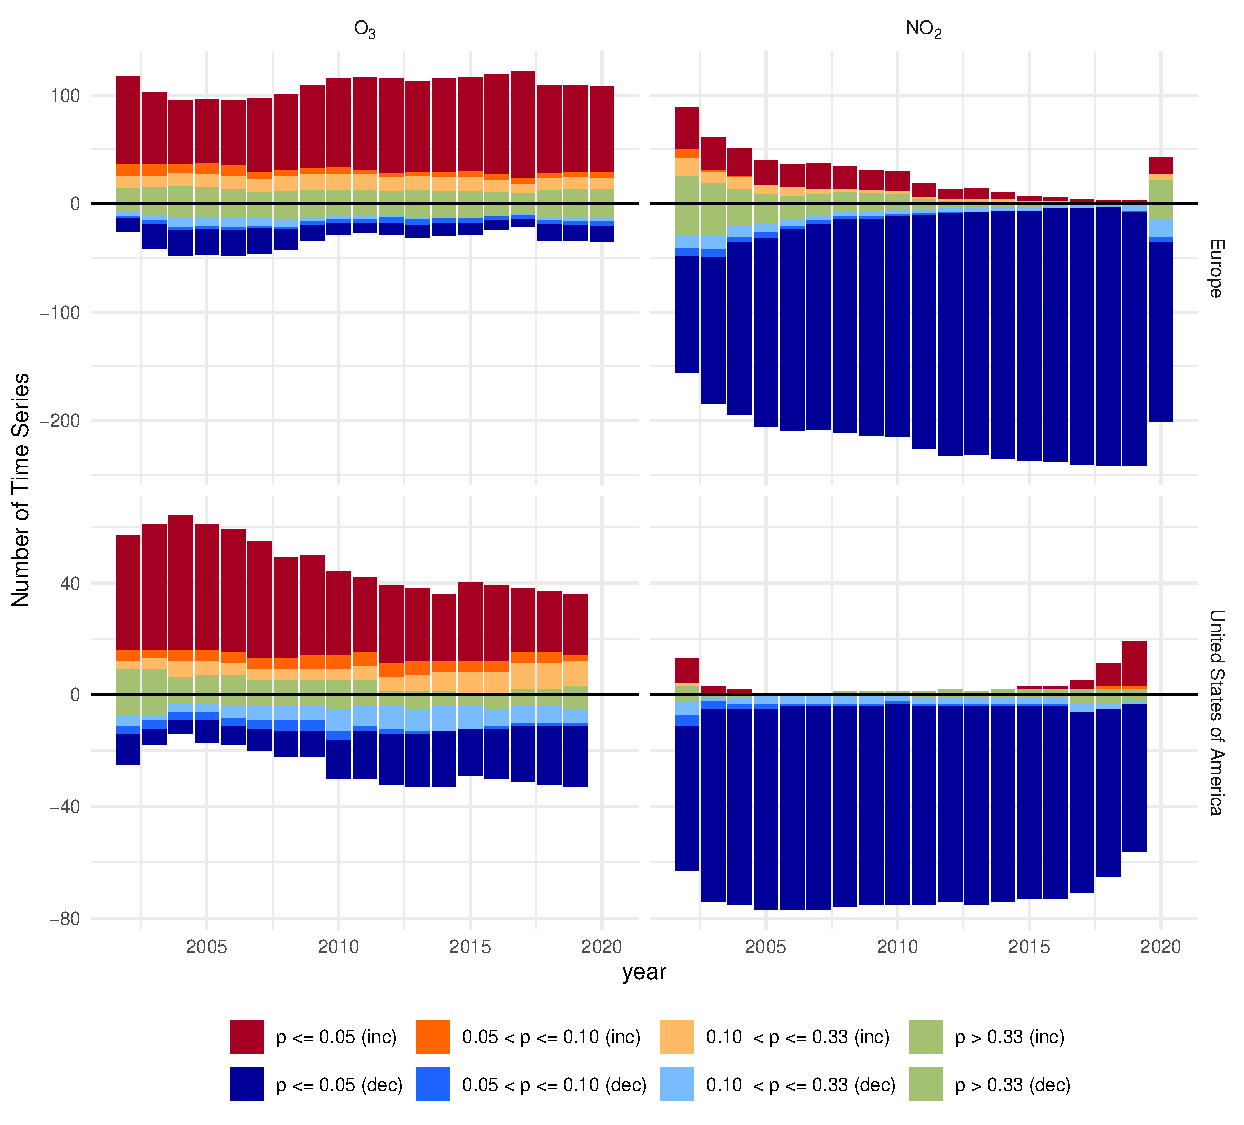
\includegraphics[width=12cm]{figures/f5_significance_bars.pdf}
\caption{Time series of trends in O\textsubscript{3} (left) and NO\textsubscript{2} (right) for Europe (top) and the USA (bottom). Positive trends are contained in the bar above 0 and negative trends are contained in the bar below 0. Colour indicates significance and direction, darkest colours being most significant (p < 0.05) and green the least (p > 0.33). Blues are decreasing trends and reds are increasing trends. In this case trends with p > 0.33 have been sorted by their direction.}
\label{fig:p_bar_year}
\end{figure*}

Figure \ref{fig:p_bar_year} counts the trends by significance and direction per year. 2000, 2001 and 2021 onward in Europe and 2000, 2001, 2020 and 2021 onwards for the USA were excluded from this year on year analysis, as it is not possible to capture changing trends in these regions due to the limitations placed on where change points can occur as detailed in section \ref{sect:method}.

This reveals the majority of trends are of high certainty. It also reinforces the observations from section \ref{sect:overview_of_trends}, where both Europe and the US see O\textsubscript{3} increasing at number of sites, with there being proportionally more sites with a decreasing trend in the US. This additionally shows that the number of high certainty decreasing trends in O\textsubscript{3} has been present since \textasciitilde{2010}, joined by a slow decline in increasing trends. 

For NO\textsubscript{2} the feature of some sites beginning to show increasing trends in the US is clear, with this pattern beginning in 2015-2016. Between 2000 and 2019 nearly all European sites moved to a trend of decreasing NO\textsubscript{2}, however, this reversed for several sites in 2020. This trend reversal can be attributed to the reduction in NO\textsubscript{2} concentrations in Europe which were a side effect of public health measures \citep{acp-20-15743-2020, acp-21-4169-2021}, and is discussed in more detail in \ref{sect:2020_in_europe}.  

\subsection{Trends Across Quantiles} \label{sect:trends_across_quantiles}

To investigate how the trends in urban O\textsubscript{3} are generally changing across quantiles in Europe and the USA, the distribution of slopes in each region was determined for each $\tau$. This section necessarily needs to discuss two sets of quantiles referring to different calculations, as such $\tau$ is used to refer to the quantile associated with the quantile regression, and other references to quantiles are associated with the analysis of the distribution of slopes within a given $\tau$.

The distributions at the start (year = 2000) and end (year = 2019) of the 20-year period were compared (Figure \ref{fig:ridgeplot}). Generally, across all values of $\tau$, the interquartile range (IQR = 75\textsuperscript{th} quantile minus 25\textsuperscript{th} quantile) of the slope distributions in O\textsubscript{3} was greater in 2000 compared with 2019 ($\tau$ = 0.5, IQR = 0.87 and 0.58 ppb yr\textsuperscript{-1} for 2000 and 2019 respectively). This is particularly true for Europe, where a clear reduction in the higher $\tau$ O\textsubscript{3} slopes is observed between 2000 and 2019. For $\tau$ = 0.95, a much larger proportion of the slopes were > 1.25 ppb yr\textsuperscript{-1} in 2000 than 2019. For $\tau$ = 0.95 in the USA, there is a reduction in the number of slopes with very negative (< 1.00 ppb yr\textsuperscript{-1}) slopes between 2000 and 2019.

\begin{sidewaysfigure}
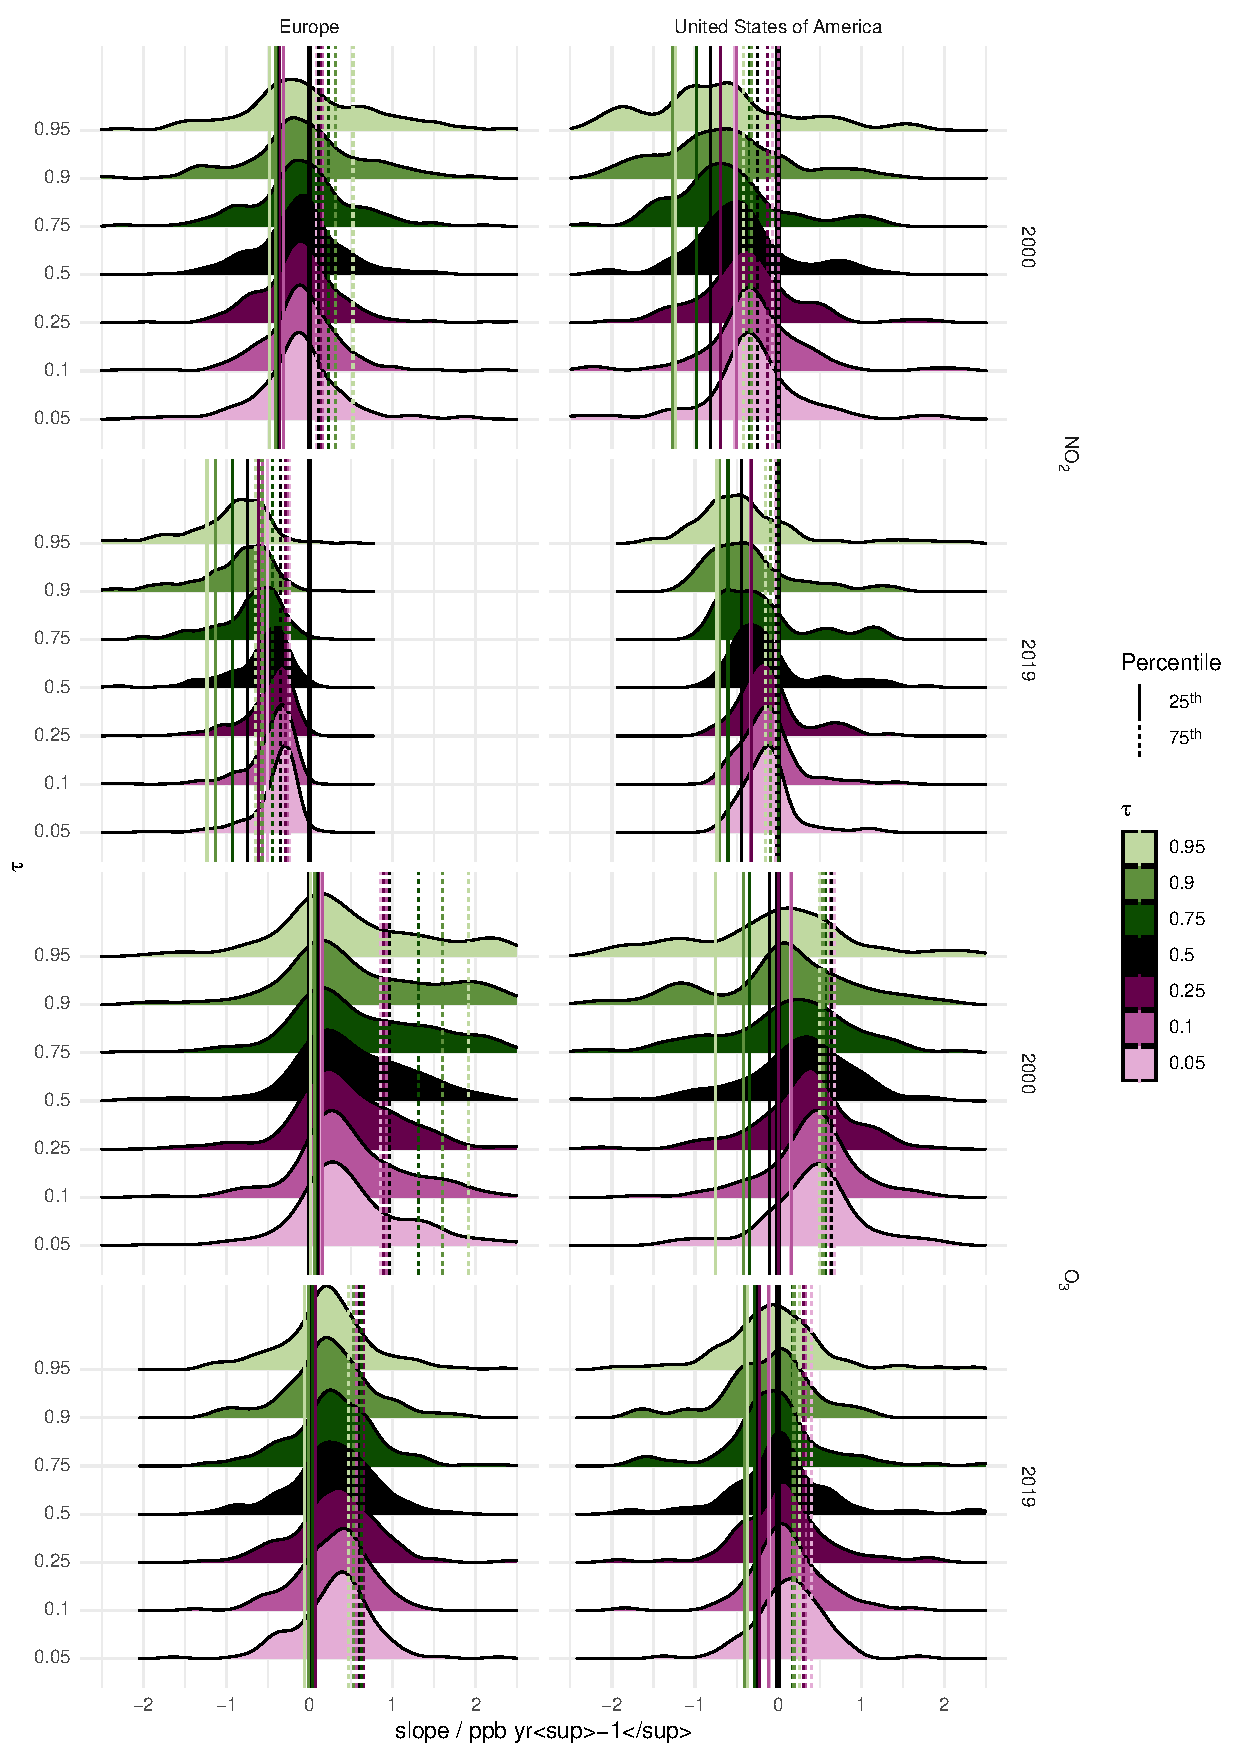
\includegraphics[height=14cm]{figures/f6_ridgelines.pdf}
\caption{Slope density for NO\textsubscript{2} (left) and O\textsubscript{3} (right) for Europe (cols 1 and 3) and the USA (cols 2 and 4) in 2000 (top) and 2019 (bottom) for $\tau$ = 0.05, 0.1, 0.25, 0.5, 0.75, 0.9 and 0.95}
\label{fig:ridgeplot}
\end{sidewaysfigure}


In Europe, the bulk of NO\textsubscript{2} slopes become more negative across all $\tau$ (Figure \ref{fig:ridgeplot}). However, in the USA, despite the majority of slopes being negative in both 2000 and 2019, there is still a proportion of slopes with positive slopes in 2019, not observed in the European distribution. This is particularly true for 0.5 >= $\tau$ <= 0.9. The IQR of the slope distributions was comparable between 2000 ($\tau$ = 0.5, IQR = 0.50 ppb yr\textsuperscript{-1}) and 2019 ($\tau$ = 0.5, IQR = 0.40 ppb yr\textsuperscript{-1}) for Europe, comparable to the reduction in spread observed in the USA in 2019 ($\tau$ = 0.5, IQR = 0.44 ppb yr\textsuperscript{-1}) compared to 2000 ($\tau$ = 0.5, IQR = 0.57 ppb yr\textsuperscript{-1}).


Annual changes in $\tau$ slopes were used to evaluate how absolute urban O\textsubscript{3} mixing ratios and trends changed across Europe and the USA between 2000 and 2021. For both Europe and the USA, the cumulative sum of the annual median of the trends across all sites was calculated for each value of $\tau$. This was followed by the subtraction of the 2000 value to get relative change since 2000. Using this analysis, Figure \ref{fig:median_slopes_per_tau_cont_name_absolute} shows the change in median O\textsubscript{3} and NO\textsubscript{2} mixing ratios since 2000. The median of these results for Europe and the United States of America was then derived for each year and for each $\tau$. From this, Figure \ref{fig:median_slopes_per_tau_cont_name_trends} describes how the magnitude and direction of the trend line changes annually.

In both Europe and the USA, median trend-derived O\textsubscript{3} mixing ratios have generally increased between 2000 and 2021 (figure \ref{fig:median_slopes_per_tau_cont_name_absolute}). This is most clearly observed in Europe, where all percentiles demonstrated a consistent increase in median O\textsubscript{3} across the two decades. Larger increases in O\textsubscript{3} were observed in the lower $\tau$ cases (+6.33 ppb, $\tau$ = 0.05) compared to the higher $\tau$ cases (+5.08 ppb, $\tau$ = 0.95), indicating that the lowest ambient O\textsubscript{3} levels are continuing to increase while higher levels show some signs of reducing their rate of increase. The picture is more mixed in the USA. Similarly to Europe, the largest increases in median O\textsubscript{3} since 2000 were observed in the lower $\tau$ cases (+4.95 ppb, $\tau$ = 0.05). In the $\tau$ = 0.50 case, median O\textsubscript{3} increased to ca. +2.5 ppb by 2011 before plateauing between 2011 and 2021. In contrast, in the highest $\tau$ value cases, median O\textsubscript{3} was lower in 2021 than in 2000 (-0.76 and -0.60 ppb, $\tau$ = 0.90 and 0.95 respectively). This suggests that higher ambient levels of O\textsubscript{3} have reduced in magnitude since 2000, compared to lower ambient levels which are continuing to increase. In both Europe and the USA, median ambient NO\textsubscript{2} mixing ratios have reduced, with the largest reductions observed in the $\tau$ = 0.95 case (-11.49 ppb and -15.94 ppb for Europe and the USA respectively). Smaller reductions were observed in the $\tau$ = 0.05 case (-4.48 and -5.78 ppb for Europe and the USA respectively).

\begin{figure*}[h!]
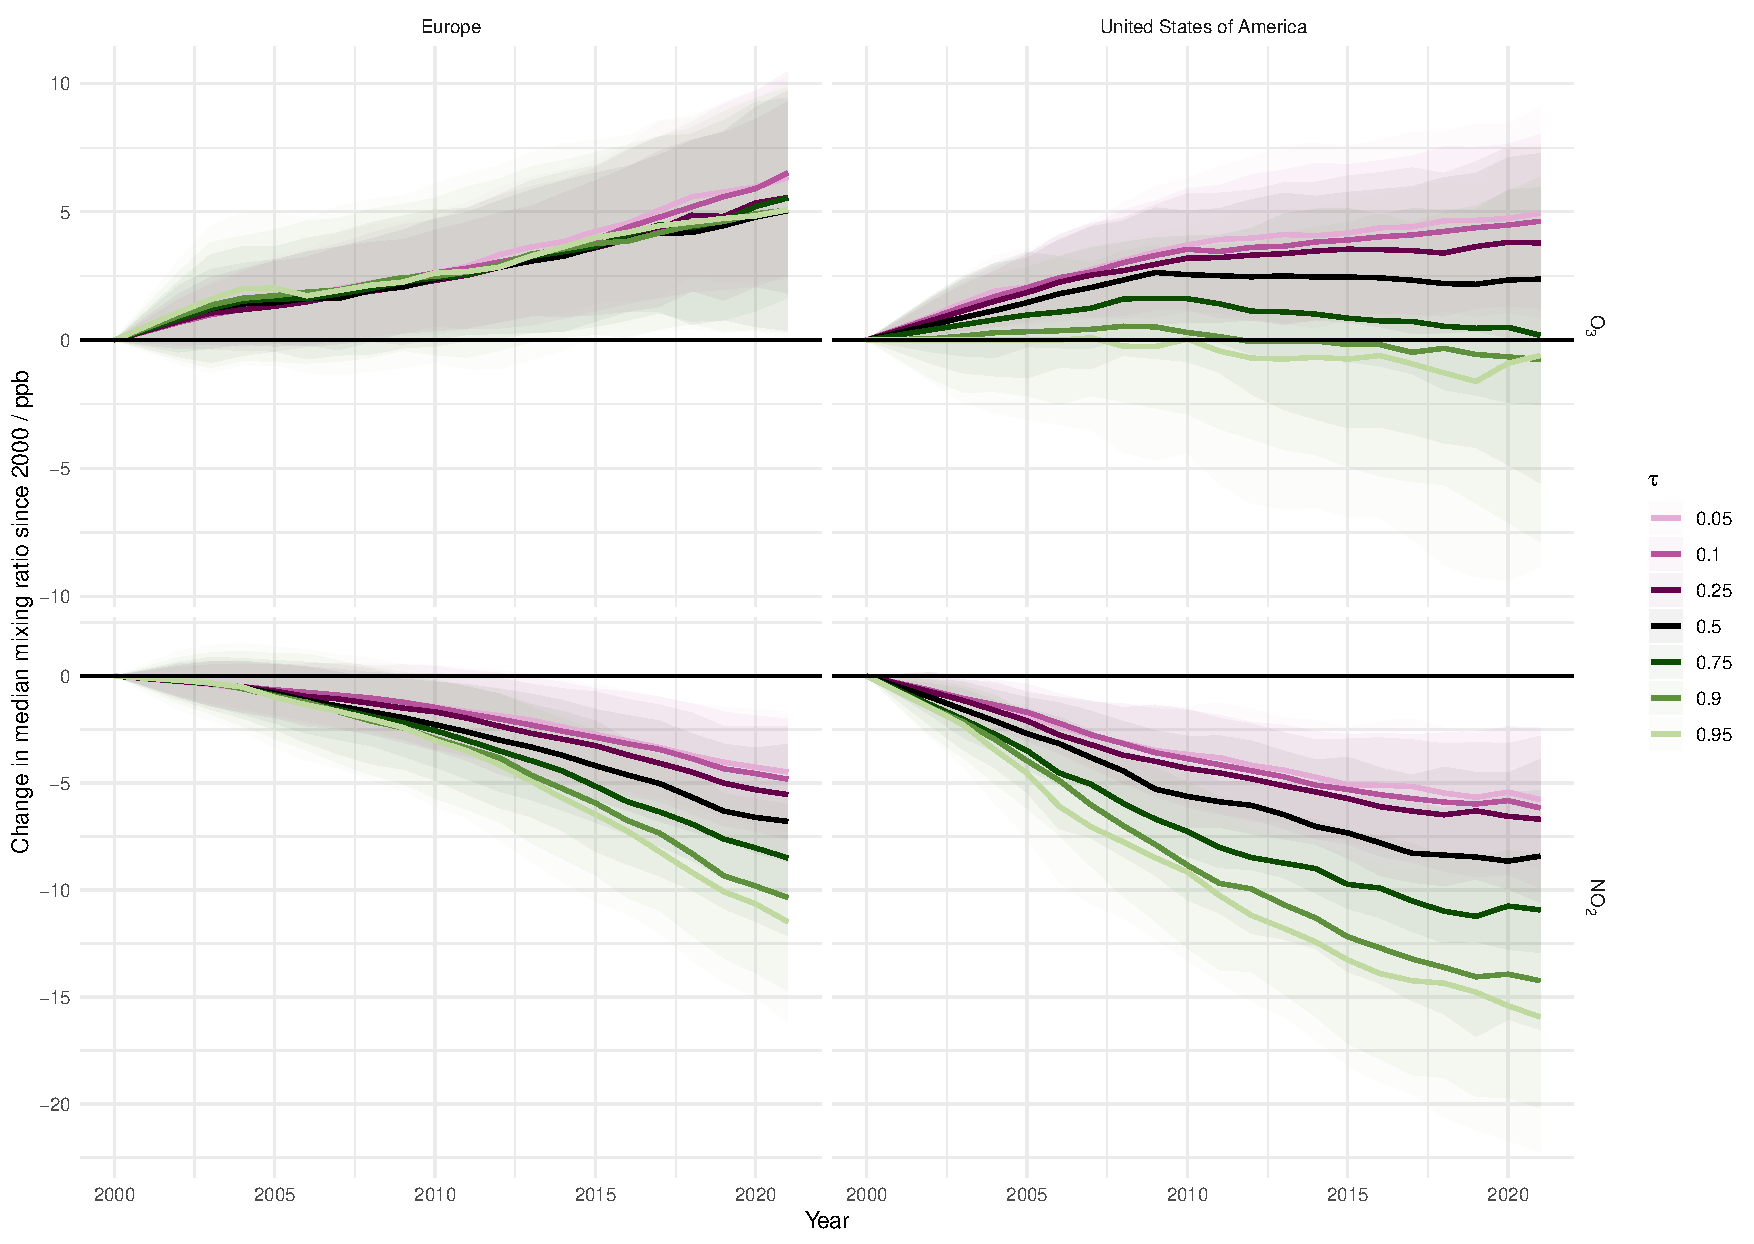
\includegraphics[width=12cm]{figures/f7_cusum.pdf}
\caption{Absolute change in trend line-derived median NO\textsubscript{2} and O\textsubscript{3} mixing ratios for Europe and the USA, coloured by trend line percentile. The shaded region represents the median absolute deviation.}
\label{fig:median_slopes_per_tau_cont_name_absolute}
\end{figure*}

Taking a closer look at the annual magnitude and direction of the trends allows for a closer inspection of how O\textsubscript{3} and NO\textsubscript{2} trends have changed between 2000 and 2021 for each $\tau$ value (Figure \ref{fig:median_slopes_per_tau_cont_name_trends}). For Europe, all median O\textsubscript{3} trends were positive for all $\tau$ values across all years. For higher $\tau$ values ($\tau$ = 0.75, 0.90 and 0.95), the slope dropped sharply from ca. 0.54 ppb yr\textsuperscript{-1} to ca 0.07 ppb yr\textsuperscript{-1} ($\tau$ = 0.95) between 2000 and 2004. A smaller decrease in slope was observed for the lower $\tau$ cases (from ca. 0.35 ppb yr\textsuperscript{-1} to 0.18 ppb yr\textsuperscript{-1} for the $\tau$ = 0.05 case). From 2005 onward, the slope in the O\textsubscript{3} trend generally continued to increase up to 2021. In the lower $\tau$ cases, the median slope returned to 2000-2002 levels in 2021. For the higher $\tau$ cases, the magnitude of the median slope was between ca. 0.29 - 0.46 ppb yr\textsuperscript{-1} lower in 2021 than 2000. In the USA, a larger spread in the changing median slopes was observed between different $\tau$ values. Generally, and in contrast to Europe, the median slope in O\textsubscript{3} steadily decreased between 2000 and 2014, before plateauing between 2014 to 2021. For the lower $\tau$ values, the slope in O\textsubscript{3} remained positive between 2000 and 2021, but reduced by ca. 0.34 ppb yr\textsuperscript{-1} between 2000 and 2014 ($\tau$ = 0.05). Trends in the higher $\tau$ cases were positive at the beginning of the century, with a transition to a negative trend observed for $\tau$ = 0.75 (in 2013), and $\tau$ = 0.90 and 0.95 (both in 2007). In the $\tau$ = 0.50 case, median trends in O\textsubscript{3} plateau around 0 ppb yr\textsuperscript{-1} from 2012, indicating no overall direction of trend.

Trends in NO\textsubscript{2} in Europe and the USA between 2000 and 2021 are also contrasting. In both Europe and the USA, median trends remain negative between 2000 and 2021, indicating NO\textsubscript{2} is decreasing in both cases, as observed in Figure \ref{fig:median_slopes_per_tau_cont_name_absolute}. However, the direction of the trend is different in each region. In Europe, the slope of the trend is becoming increasingly more negative with time, particularly for the higher $\tau$ cases (reduction of ca. 0.72 ppb yr\textsuperscript{-1} for the $\tau$ = 0.95 case). However, in the USA the negative trends are becoming increasingly more positive (or less negative) between 2000 and 2021 (0.29 ppb yr\textsuperscript{-1} higher, $\tau$ = 0.95). 

%Interestingly, in both cases, although important changes in the direction of the trend are observed for O\textsubscript{3} and NO\textsubscript{2}, there is no clear change in trend for O\textsubscript{x} despite a clear reduction in its absolute median mixing ratio (Figure \ref{median_slopes_per_tau_cont_name_absolute}). For all $\tau$ values, O\textsubscript{x} trends are negative and consistent in magnitude for each $\tau$ value. The exception to this is observed in Europe between 2000 - 2003 where the O\textsubscript{x} trend switches sharply from being positive (ca. +1.16 ppb yr\textsuperscript{-1}, $\tau$ = 0.95) to negative (-0.16 ppb yr\textsuperscript{-1}, $\tau$ = 0.95). The O\textsubscript{x} trend then remains negative, and consistently < 0.25 ppb yr\textsuperscript{-1} in most $\tau$ cases (excluding $\tau$ = 0.95) between 2004 - 2021, and including the $\tau$ = 0.95 case from 2009 onward.

\begin{figure*}[t]
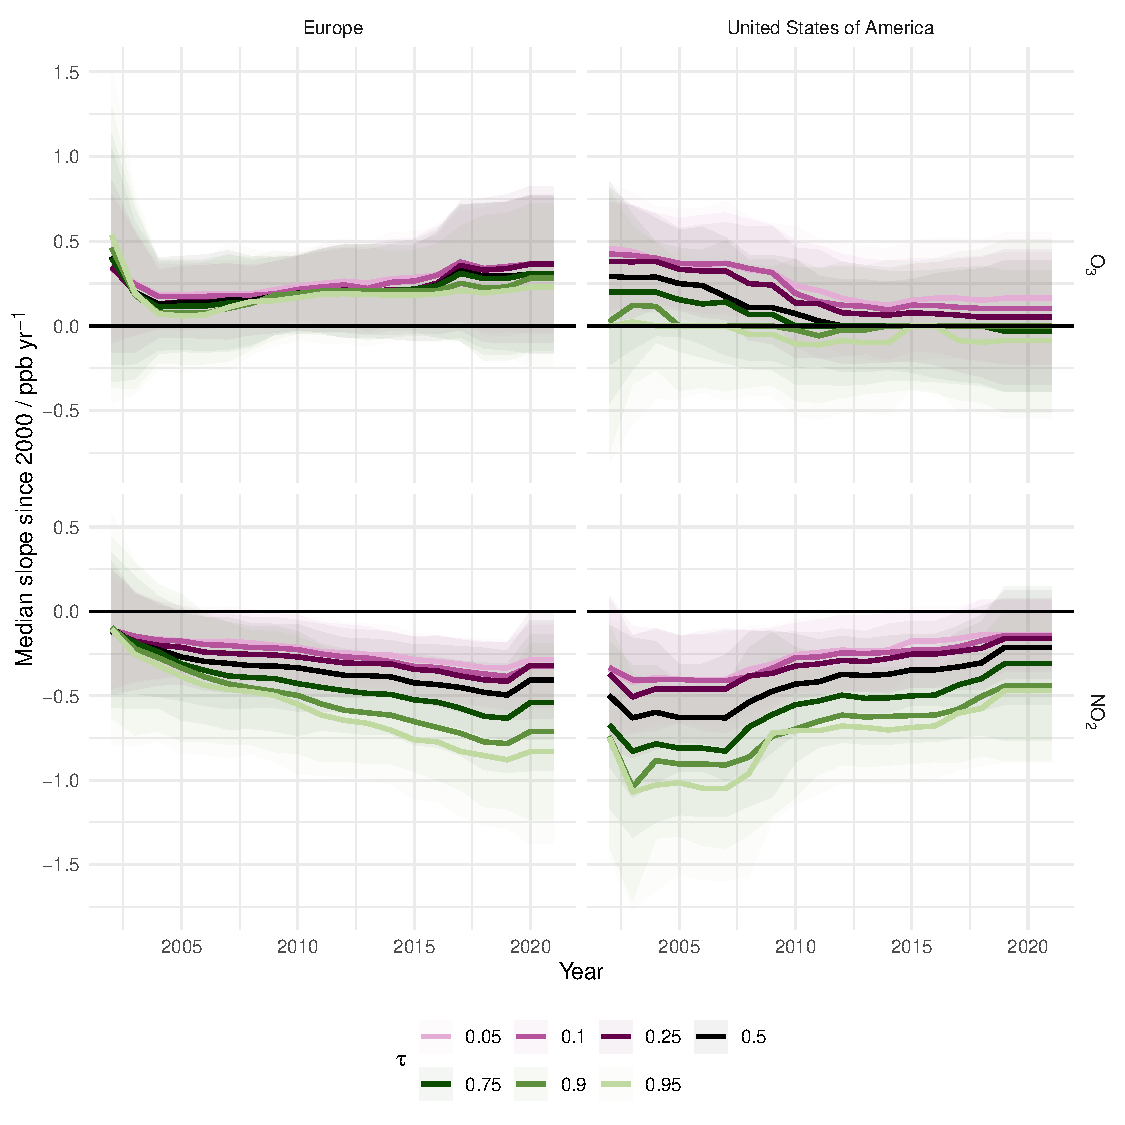
\includegraphics[width=12cm]{figures/f8_slopes.pdf}
\caption{Median trend line slopes (ppb yr\textsuperscript{-1}) in NO\textsubscript{2} and O\textsubscript{3}  for Europe and the USA, coloured by trend line $\tau$ value. The shaded region represents the median absolute deviation.}
\label{fig:median_slopes_per_tau_cont_name_trends}
\end{figure*}

\clearpage

\subsection{Spatio-temporal Distribution of Change points} \label{sect:case_studies}

% So the Flemming paper looked at 4MDA8 levels, and there were hotspots in California and southern Europe (in particular, northern Italy and Greece... how do we tie this in with our trend analysis without looking at MDA8?

The direction and magnitude of the change points in each location were investigated to identify locations where a change in direction of the trend (i.e. a negative to positive trend) occurs. In Europe, 21 sites observed a switch from a negative O\textsubscript{3} trend line to a positive one in the first change point. The biggest switches occurred in southern Europe, in Spain and Greece ($\Delta$3.28 ppb in \textit{gr0022a}, 2004). For a larger number of sites (41), mainly in central Europe, the first change point in O\textsubscript{3} switched from positive to negative, up to a maximum swing of 4.55 ppb (\textit{fr31013}, 2003). In contrast, a larger number of sites observed a negative to positive switch (39) in the second change point, compared to a positive to negative switch (28). Eight of the top ten biggest switches from negative to positive in the second change point occurred in Spain and Italy ($\Delta$3.99 ppb in \textit{es0124a}), whereas the biggest switch from positive to negative showed no distinct spatial pattern. This suggests that generally across Europe, more trends in O\textsubscript{3} were switching from positive to negative in the first 5-10 years of the 21st-century, whereas more trends were switching from negative to positive between 2010-2021. In both decades, southern European sites showed the biggest changes in O\textsubscript{3} trend from negative to positive.
Similarly to O\textsubscript{3}, more sites showed a positive to negative trend (84) in NO\textsubscript{2} compared to negative to positive (28) for the first change point, with the largest change points again observed in Spain ($\Delta$3.25 ppb, \textit{es1453a}). A comparable number of sites showed changes in trend direction in the second change point, (43 negative to positive, and 33 positive to negative). The positive to negative trends were generally distributed around 2010-2014, whereas the vast majority of negative to positive switches occurred in 2020 (41 out of 43 sites). The cause of this switch in 2020 across Europe is discussion in further detail in section \ref{sect:2020_in_europe}.

\begin{figure}[p]
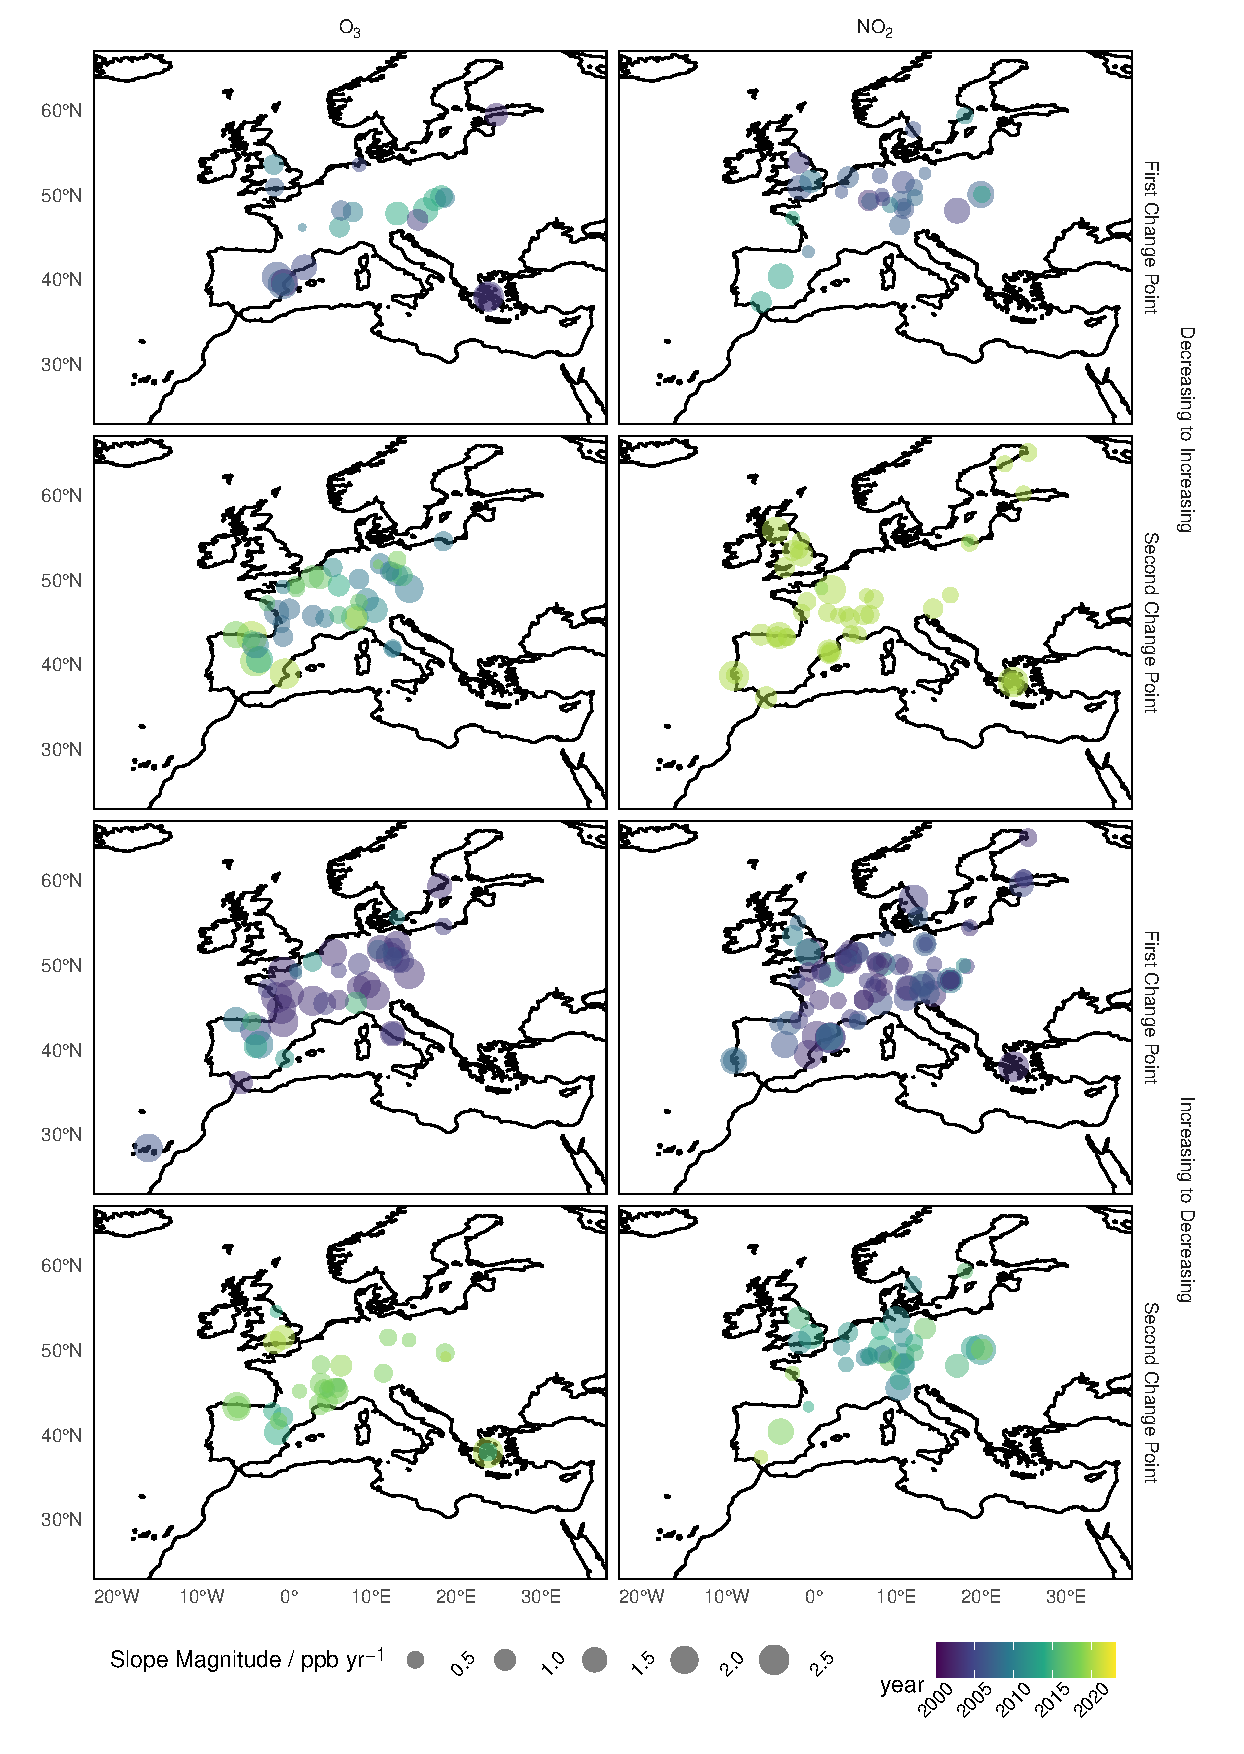
\includegraphics[width=12cm,keepaspectratio]{figures/f9_eu_mag_map.pdf}
\caption{European sites with a change in direction of slope (O\textsubscript{3} - left, NO\textsubscript{2} - right) of the first (rows 1, 3) second (rows 2, 4) change points. The size of the slope is relative to the magnitude of the change in slope (slopes > 2.5 ppb yr\textsuperscript{-1} have been clamped), coloured by the year of the change point. Negative to positive change points (rows 1, 2) are presented separately to positive to negative change points (rows 3, 4).}
\label{fig:eu_changepoint_map}
\end{figure}

\begin{sidewaysfigure}
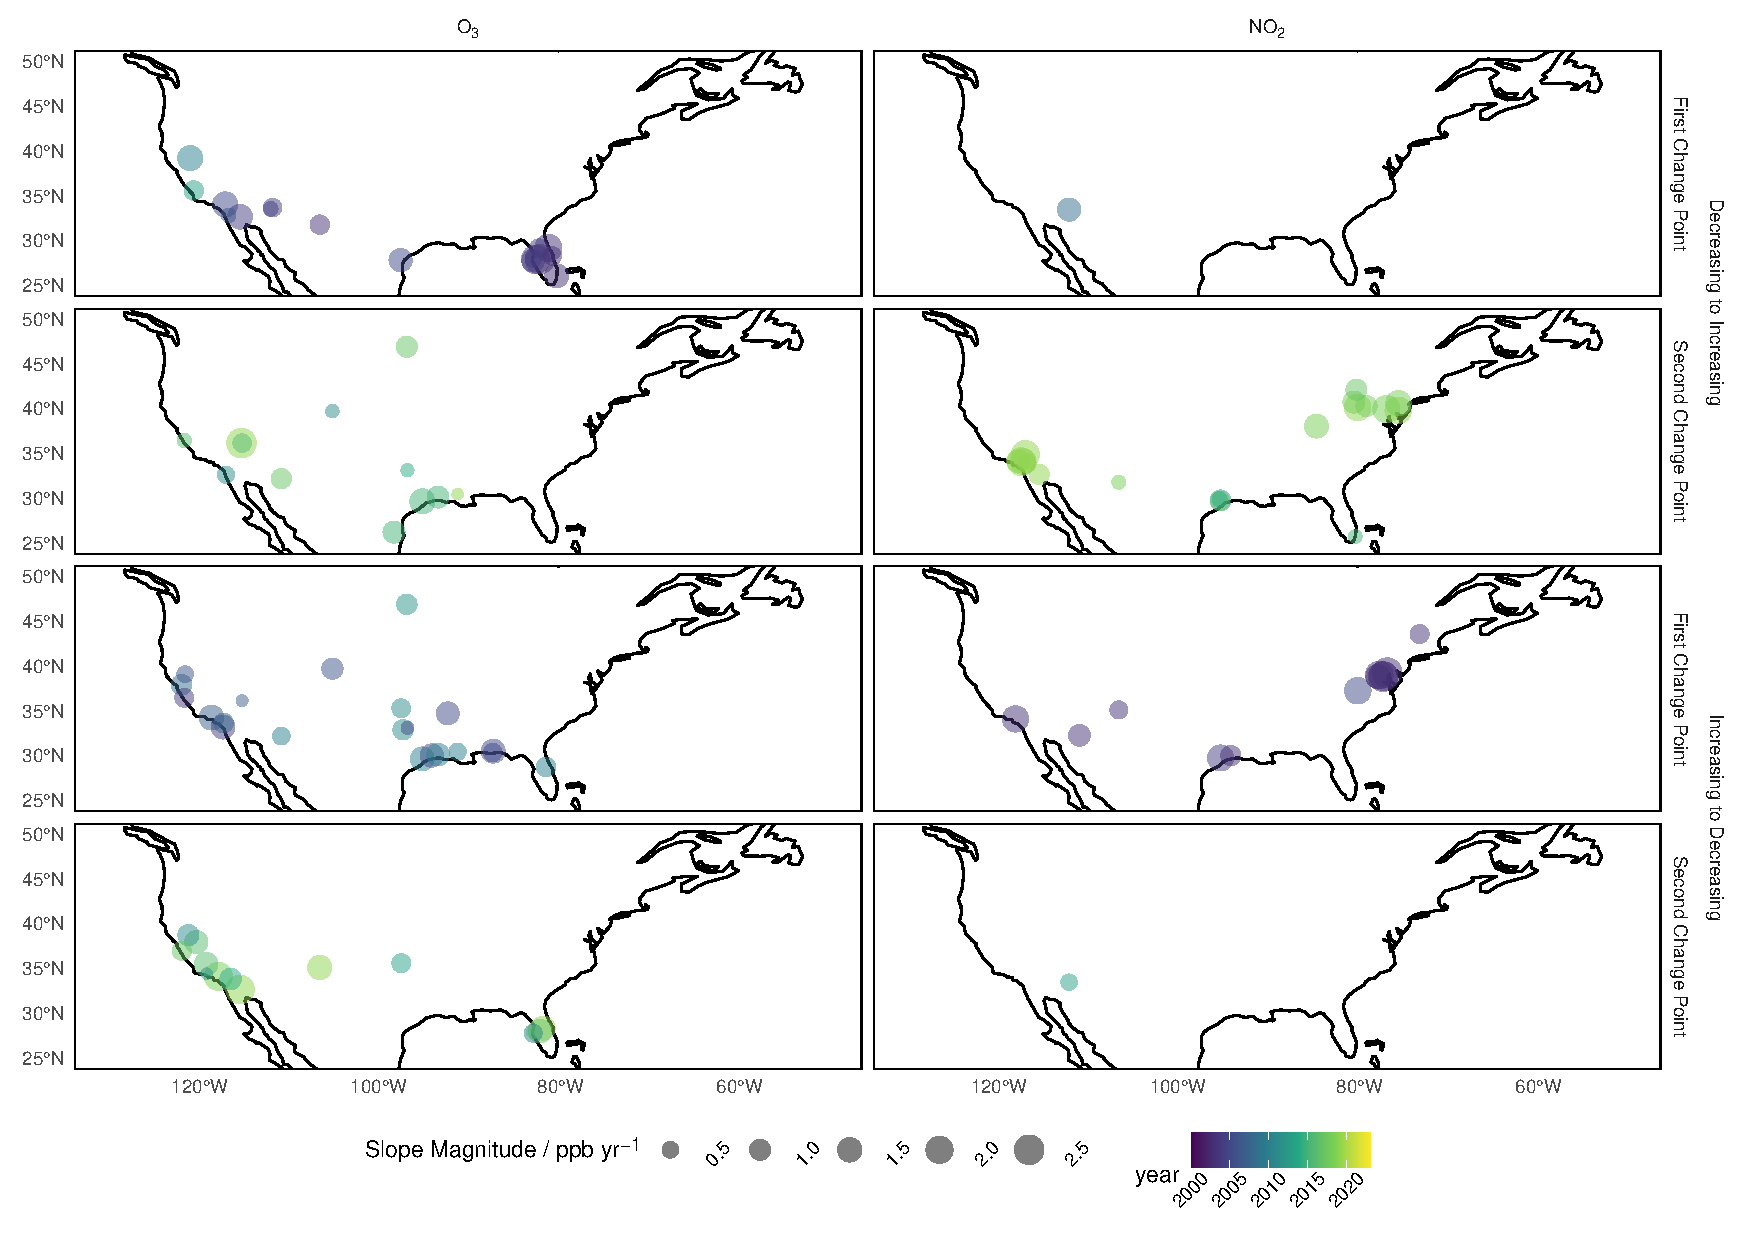
\includegraphics[height=14cm]{figures/f10_us_mag_map.pdf}
\caption{US sites with a change in direction of slope (O\textsubscript{3} - left, NO\textsubscript{2} - right) of the first (rows 1, 3) second (rows 2, 4) change points. The size of the slope is relative to the magnitude of the change in slope (slopes > 2.5 ppb yr\textsuperscript{-1} have been clamped), coloured by the year of the change point. Negative to positive change points (rows 1, 2) are presented separately to positive to negative change points (rows 3, 4).}
\label{fig:us_changepoint_map}
\end{sidewaysfigure}

In the USA, a comparable number of directional switches in O\textsubscript{3} trend in the first change point occurred in the positive to negative direction (21), compared to negative to positive (17). The three largest magnitude trend changes from negative to positive occurred in Florida ($\Delta$2.43 ppb, \textit{15292}), with all of the ten highest magnitude cases in either Florida or California. Trends switching from positive to negative in the first change point scenario were smaller in magnitude, the biggest switch being in California ($\Delta$1.53 ppb, \textit{8197}), but with some noticeable contributions from the central states. The majority of second change points occurred between 2010-2019, though it is important to note that due to a lack of data availability, it is not possible for this analysis to pick out change points from 2020 onward in the USA dataset. In total, 14 sites switched from positive to negative, with a maximum change of $\Delta$2.25 ppb (\textit{8169}, 2019). A comparable number of sites (12) showed trends switching from negative to positive, with a maximum change of $\Delta$2.46 ppb (\textit{1959}, 2019). In the NO\textsubscript{2} dataset, there is only one site showing a switch from negative to positive in the first change point ($\Delta$1.30 ppb, \textit{1369}, 2008), compared to 13 sites showing a positive to negative switch. Of these 13 sites, the largest magnitude is in Virginia ($\Delta$2.99  ppb, \textit{15024}, 2003). In contrast, 19 sites show a switch in NO\textsubscript{2} trend from negative to positive after the second change point, with the biggest change in California ($\Delta$2.16 ppb, \textit{1206}, 2019), with only one site showing a switch from positive to negative ($\Delta$0.48 ppb, \textit{1369}, 2013).

Generally, the largest changes from negative to positive O\textsubscript{3} trends in the USA were in California and Florida in the first half of the 20 year period, with the reversal of this trend seen across California and Florida in the second change point. 8/14 and 4/14 of the sites showing a positive to negative transition in the second change point were located in California and Florida respectively. This is important, since a previous study highlighted that 4th highest daily maximum 8-hour O\textsubscript{3} (4MDA8) values between 2010-2014 were particularly high in California \citep{fleming_2018}. 

To supplement this analysis, the 4MDA8 was calculated using the mixing ratio data for each site and slicing the fourth highest value on an annual basis. 4MDA8 is an important metric used by the US for determining compliance with the National Ambient Air Quality Standards for Ozone \citep{EPA_2015, Berrocal_4MDA8}. To allow for comparison with previous studies, only the 6-month warm season (April - September) was used to calculate 4MDA8 values, which is a reasonable approach in the USA and Europe since the highest O\textsubscript{3} values are likely to occur in the warmest months.

Figure \ref{fig:us_4mda8_map} shows how the 4MDA8 value varies between 2000, 2007, 2014 and 2021 in the USA. Across the US, 33 sites had a 4MDA8 >= 85 in 2000, compared to 19 in 2007 and 6 in 2014. In 2016 there was an up-tick to 10 sites with 4MDA8 values at this level. Of these 10 sites, all are located in California, compared to 20/33 Californian sites in 2000 and 18/19 in 2007. All 11 sites in 2021 with 4MDA8 >= 85 were located in California. This highlights that although fewer Californian sites are exceeding 4MDA8 >= 85 ppb with time over the 2-decade period, the Californian 4MDA8 "hotspot" identified in \cite{fleming_2018} is still present. The more general picture across the USA is that 4MDA8 values are coming down with time, particularly strongly in the central and Eastern portion of the USA but less successfully in the west.

\begin{figure*}[h]
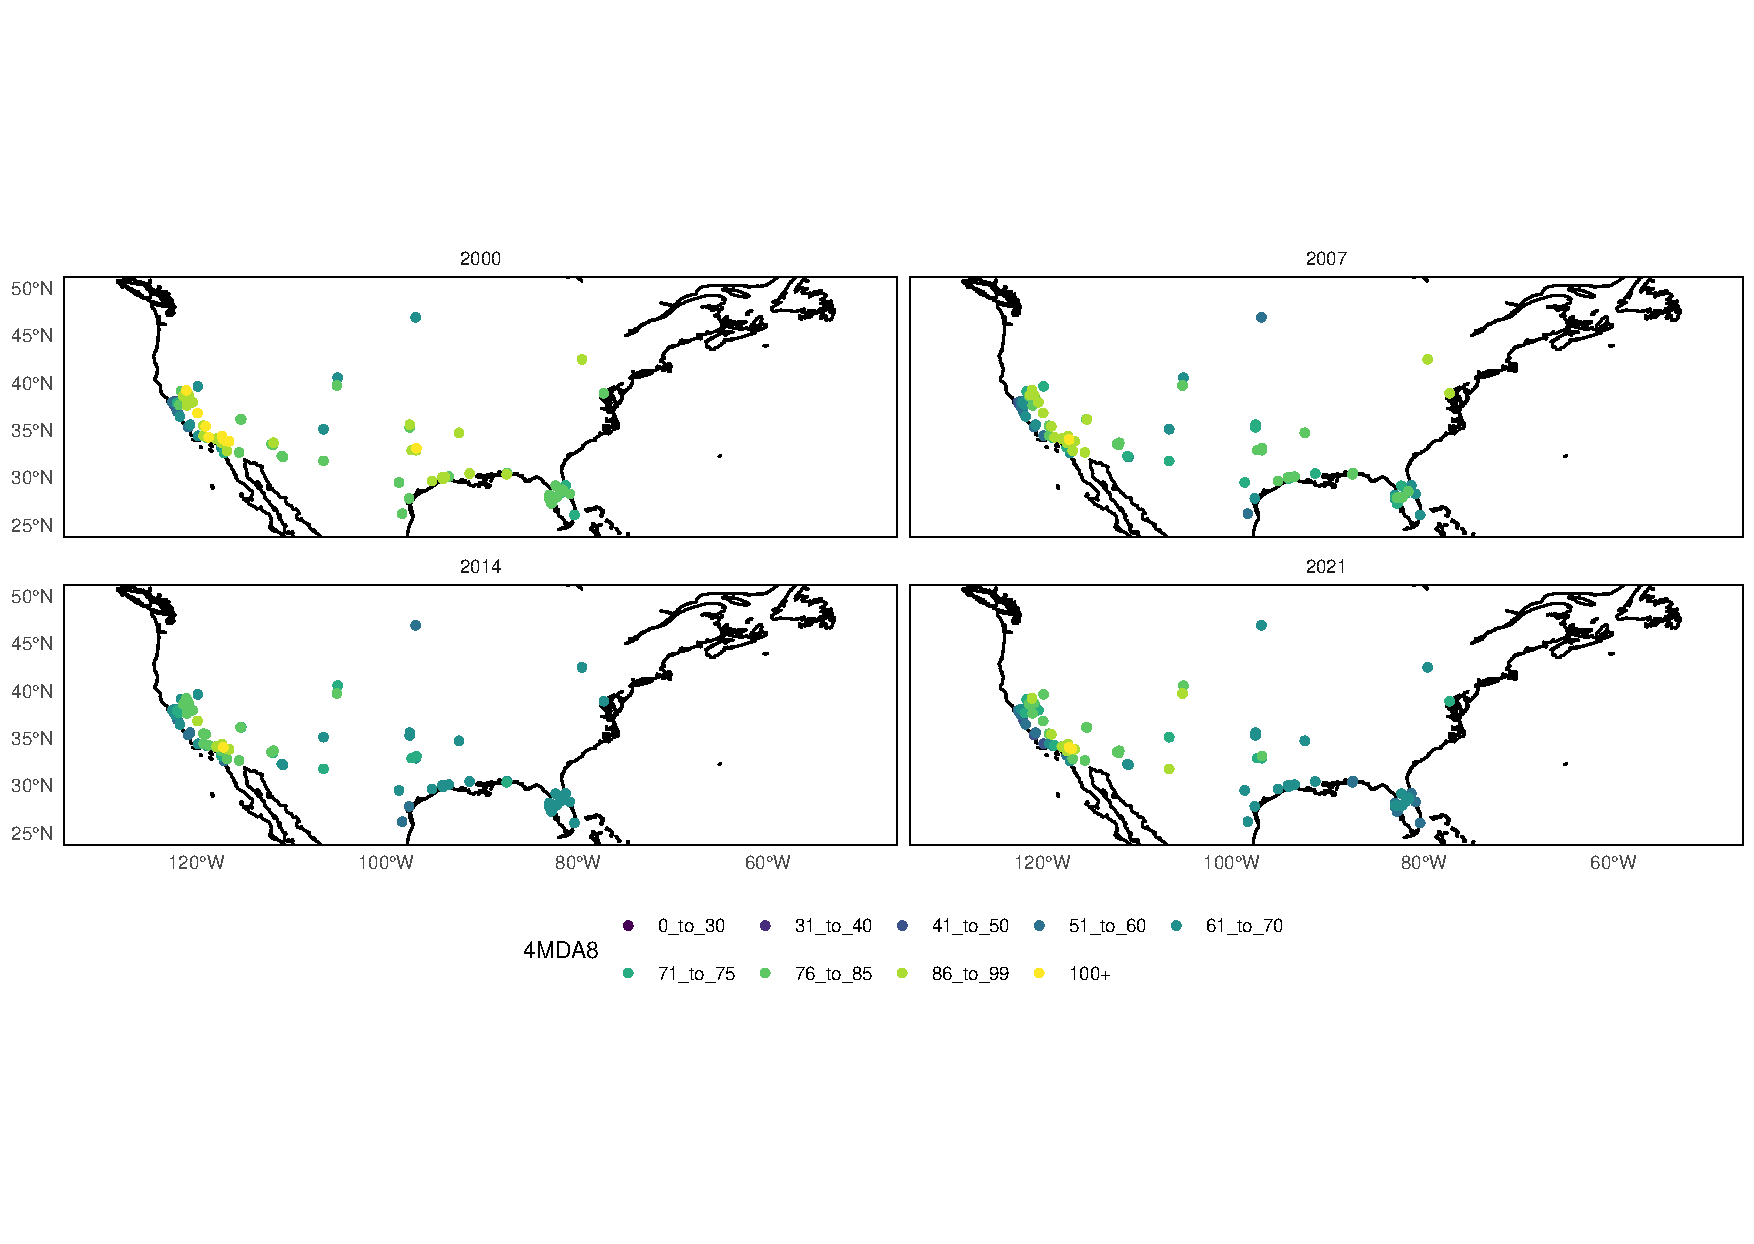
\includegraphics[width=12cm]{figures/f11_4mda8_us.pdf}
\caption{4MDA8 values in ppb for sites in the United States in 2000, 2007, 2014 and 2021}
\label{fig:us_4mda8_map}
\end{figure*}

Southern Europe, particularly Greece and Northern Italy, were also highlighted in \cite{fleming_2018} as being 4MDA8 hotspots. Figure \ref{fig:eu_4mda8_map} shows how the 4MDA8 values are changing between 2000, 2007, 2014 and 2021 across Europe. In 2000, there were 6 sites in which 4MDA8 >= 85 ppb. This slightly increased to 7 sites in 2007 before decreasing to 4 sites in 2014. By 2021, no sites had 4MDA8 values exceeding 85 ppb. Since the measurement sites in this dataset are not evenly distributed across the USA and Europe, it is difficult to attribute high 4MDA8 values to particular states or countries, However, it was noticeable that a large proportion of the sites were 4MDA8 >= 85 ppb were in Italy and Greece. In 2000 3/6 of high 4MDA8 sites were located in Italy, and 1/6 in Greece. In 2007, 3/7 were located in Italy and 1/7 in Greece; and in 2014 3/4 sites were located in Italy. Consistent with the \cite{fleming_2018} study, the southern European 4MDA8 hotspots are apparent throughout the 20-year period. 

\begin{figure*}[h]
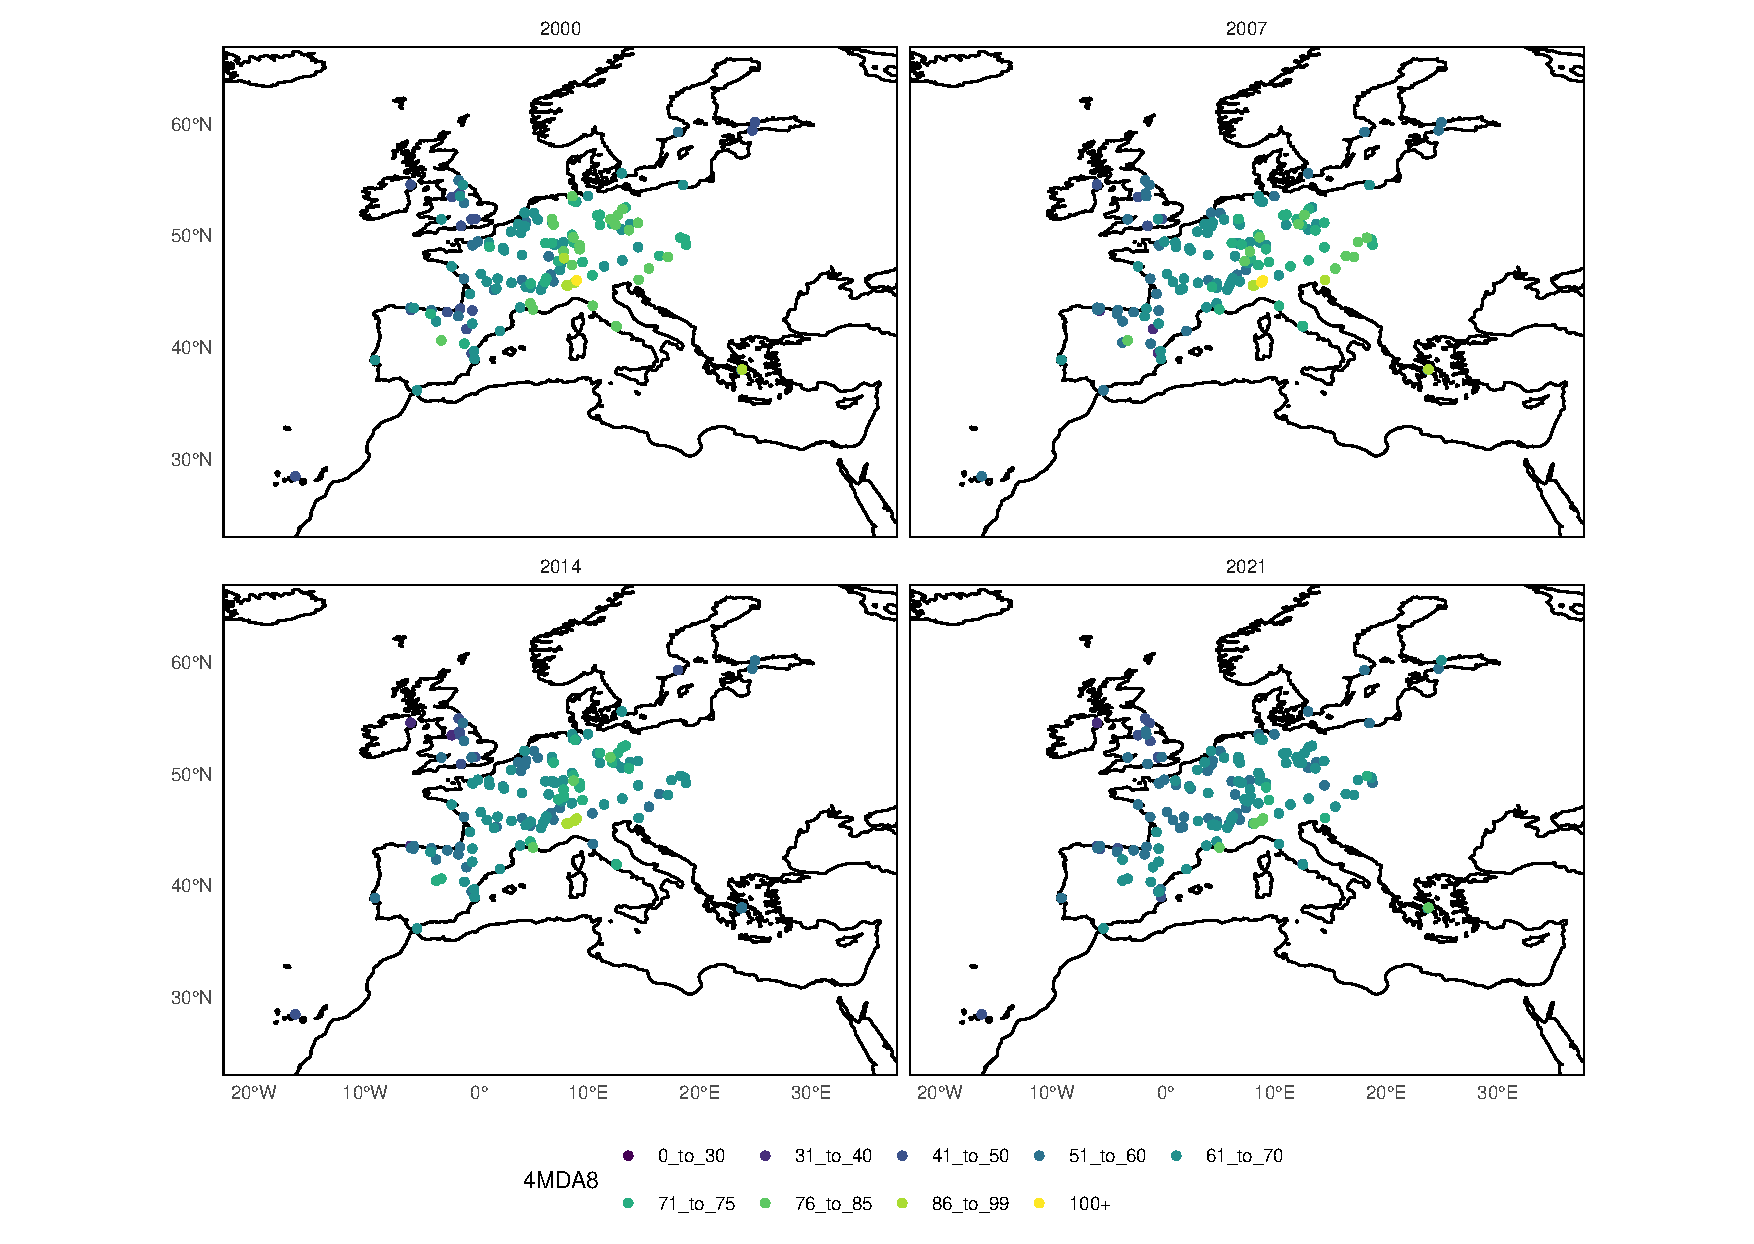
\includegraphics[width=12cm]{figures/f12_4mda8_eu.pdf}
\caption{4MDA8 values in ppb for sites in Europe in 2000, 2007, 2014 and 2021}
\label{fig:eu_4mda8_map}
\end{figure*}

\subsubsection{2020 In Europe} \label{sect:2020_in_europe}
As noted in section \ref{sect:significance_of_trends}, in 2020 in Europe several sites switched from a long term decrease in NO\textsubscript{2} to increasing NO\textsubscript{2} again. The public health measures enacted due to the COVID-19 pandemic had the side effect of decreasing NO\textsubscript{2} concentrations due to reduced traffic emissions. The removal of these measures led to an increase in NO\textsubscript{2} mixing ratios as normal activities resumed, resulting in a positive trend in NO\textsubscript{2} concentrations up from their lowest during the restrictions. There are 42 sites that had a negative trend in 2019 and a non-negative trend in 2020. The 2019 trends ranged from 1.47 to -0.04 ppb yr\textsuperscript{-1} and the 2020 trends ranged from 0.00 to 3.74 ppb yr\textsuperscript{-1}. There were two sites that already had non-negative trends (\textit{fr25039} and \textit{pl0048a}) by 2020, but neither were strong or significant (p > 0.33). 
The effect of this on O\textsubscript{3} concentrations at the sites is varied.  21 of the 42 sites also measured O\textsubscript{3}, though only 3 (\textit{es1038a}, \textit{fr33120} and \textit{gr0031a}) also had 2020 as one of the change points for the PQR. To compare the 2020 onwards trends, new PQRs for each site were selected by requiring the second change point to occur in 2020, and then selecting where the first occurred on a time series by time series basis by minimising the AIC as before. Furthermore, only sites where the resulting slope for the 2020 onwards O\textsubscript{3} trend had p values < 0.33 were selected. One final site (\textit{gr0031a}) was removed as although it meets the data coverage criteria for the main analysis, its missing data is focused around 2019 and 2020 which has a strong influence on the trends derived. This led to 15 sites remaining for this case study. 
The resulting alternative trends for these sites are shown in figure \ref{fig:2020_in_europe}. Additionally, as the focus is on sites with both NO\textsubscript{2} and O\textsubscript{3}, O\textsubscript{x} is displayed. If a site is under a VOC limited regime, the trend in O\textsubscript{x} provides an indication whether any changes in O\textsubscript{3} are only due to changes in NO\textsubscript{2}, or other factors. Whether a change in NO\textsubscript{2} concentrations results in an increase or decrease in O\textsubscript{3} concentrations depends on the if a site is sensitive to locally produced O\textsubscript{3} (which an urban site, in general, would be expected to be), and what photochemical regime (NO\textsubscript{x} or VOC limited) the site is under. For example, in a VOC limited regime, if NO\textsubscript{2} increases, O\textsubscript{3} decreases but O\textsubscript{x} remains the same, the change in O\textsubscript{3} can be attributed to the change in NO\textsubscript{2}. If NO\textsubscript{2} and O\textsubscript{3} increase, O\textsubscript{x} will also increase, indicating a NO\textsubscript{x} limited regime.
14 of the sites saw increasing O\textsubscript{3} with increasing NO\textsubscript{2} between 2020 and 2023 - this is expected in NO\textsubscript{x} limited regimes. Due to the need for both O\textsubscript{3} and NO\textsubscript{2} to be measured at both sites 13 of the sites were urban background and 2 were urban traffic, as O\textsubscript{3} is less frequently measured at traffic sites. Urban background sites are more likely to be under NO\textsubscript{x} limited regimes as they are, by design, situated further from major roads, which are still a significant source of NO\textsubscript{x}. This does not necessarily mean that urban areas in Europe are completely NO\textsubscript{x} limited and will depend on the specific location as to whether an urban traffic or urban background site is more representative of a location. At one urban traffic site (\textit{es1529a}) has seen decreasing O\textsubscript{3} with increasing NO\textsubscript{2} over the same period. This is more indicative of a VOC limited regime, and is more similar to the overall trends seen across Europe in the 21\textsuperscript{st} century, with more increasing O\textsubscript{3} trends in 2015-2021 than in 2000-2004. 

The sites identified by this method do not appear to have resumed their pre-2020 trends, though this should be verified when sufficient data has been collected post-2020 where change points will have more freedom to occur. The pattern of sites switching to an increasing trend in NO\textsubscript{2} will have varied effects on urban O\textsubscript{3} in Europe if they continue, though as background sites are designed to be more representative of residential areas, which make up a large portion of urban areas then it could be expected to see urban O\textsubscript{3} continue to increase. 


\begin{sidewaysfigure}
    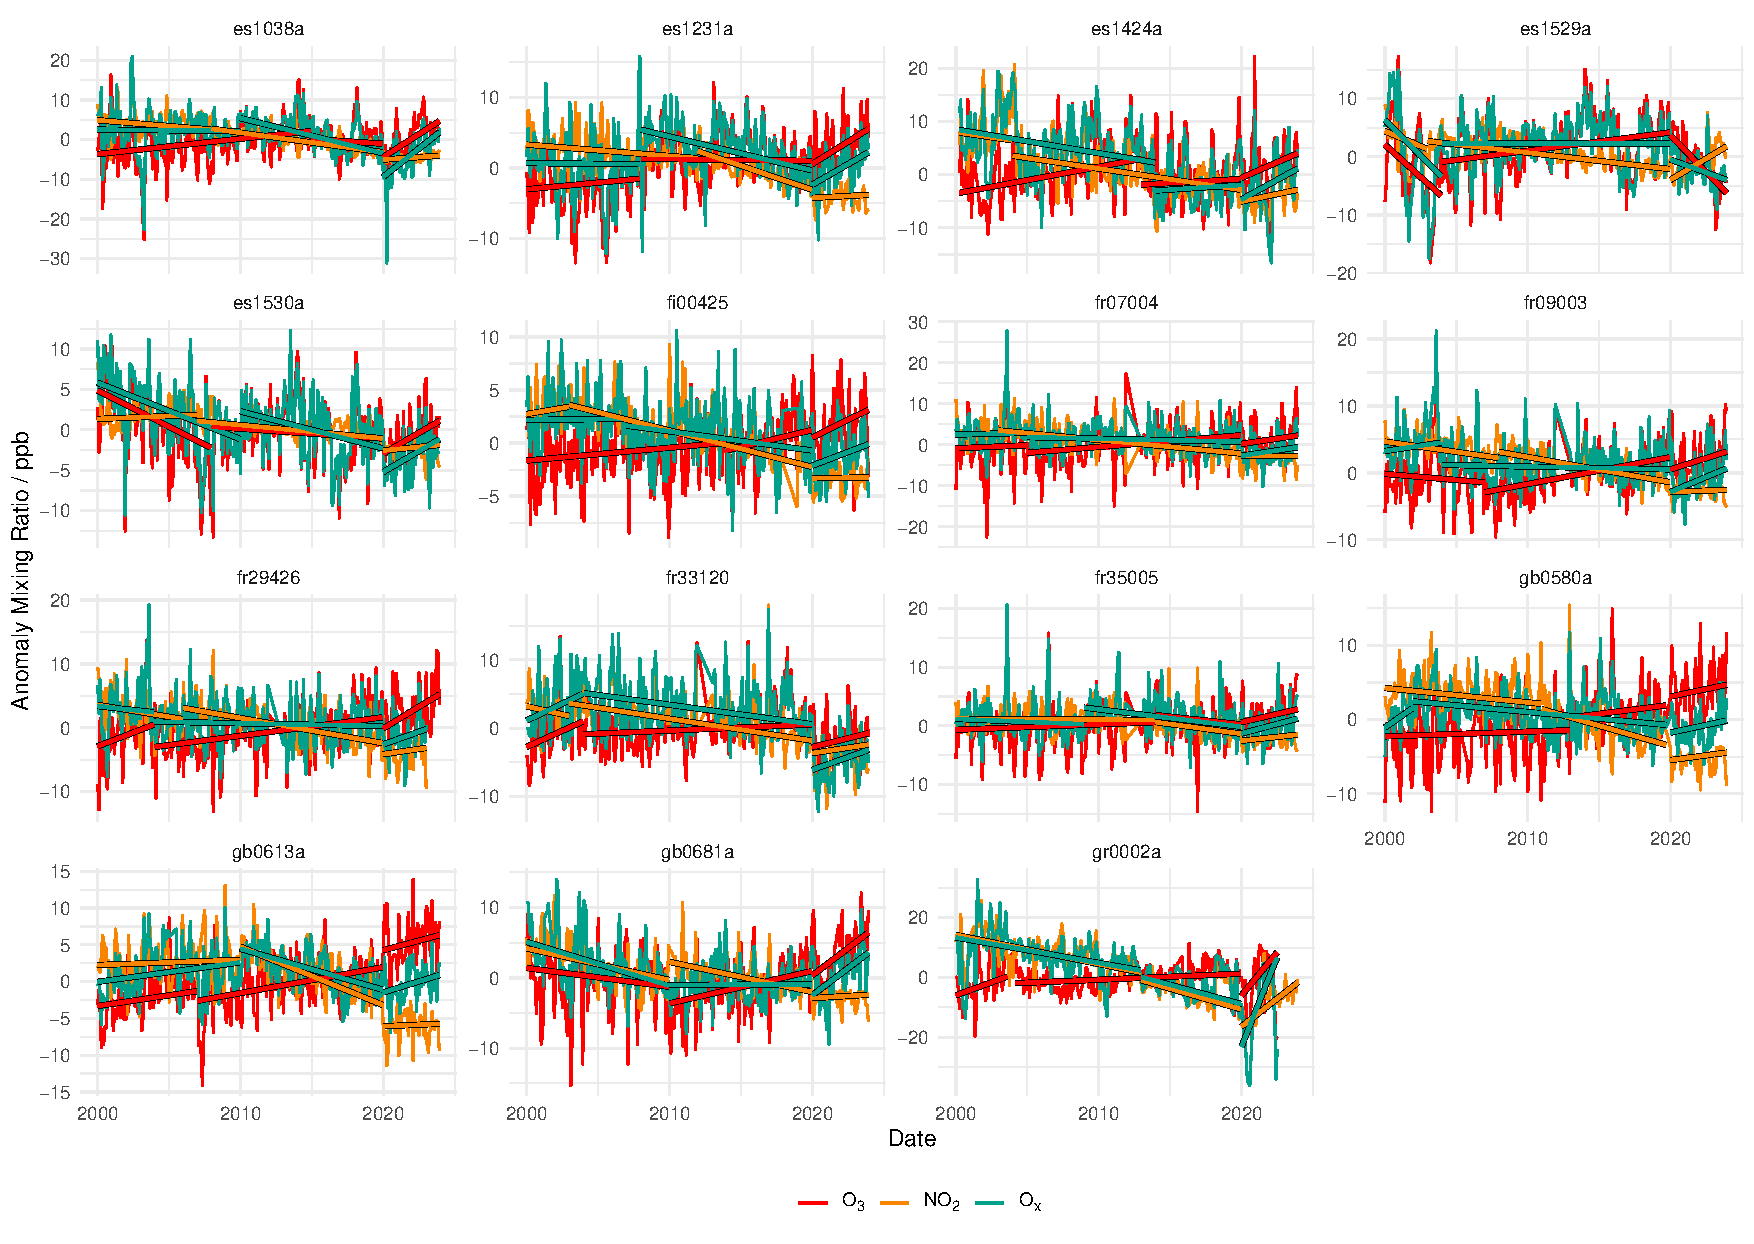
\includegraphics[height=14cm]{figures/f13_2020_in_europe.pdf}
    \caption{Sites in Europe that had decreasing NO\textsubscript{2} in 2019 but increasing NO\textsubscript{2} from 2020 onwards. Monthly averaged O\textsubscript{3} (red), NO\textsubscript{2} (orange) and O\textsubscript{x} (green) anomaly are shown. O\textsubscript{3} and O\textsubscript{x} trends differ from those presented elsewhere in the manuscript as the piecewise quantile regression where the second change point has been restricted to be in 2020.}
    \label{fig:2020_in_europe}
\end{sidewaysfigure}

\subsubsection{Recent NO\textsubscript{2} in the USA} 
In the final years of the USA NO\textsubscript{2} dataset, an up-tick the number of positive NO\textsubscript{2} trends can be seen. From 2015 onwards there is an increasing number of sites with this trend reaching 17 sites trends (16 high, 1 medium certainty) in 2021, up from 0 in 2014. Anomaly time series and trends of can be viewed in figure \ref{fig:no2_in_usa}. Trends have reversed from -0.98 - -0.03 ppb yr\textsuperscript{-1} to 0.1 - 1.78 ppb yr\textsuperscript{-1}. Unfortunately, only 4 of the 17 sites have concurrent measurements of O\textsubscript{3} so it is difficult to investigate this changing trend in NO\textsubscript{2} from the time series analysed in this study. Only one site (8169) O\textsubscript{3} trend has its original second change point occurring alongside its NO\textsubscript{2} increasing change point, so the same method has been applied as in \ref{sect:2020_in_europe} where the second change point has been forced to occur in the same year as the NO\textsubscript{2} change point. Doing this reveals that sites 8169, 14386 and 15197 have reasonably significant (p = 0.01, 0.15, 0.002 respectively) O\textsubscript{3} trends after change point 2, when this change point is the same as that in NO\textsubscript{2}. 8169 and 14386 have decreasing O\textsubscript{3} trends (-1.70 and -0.55 ppb yr\textsuperscript{-1}) with increasing NO\textsubscript{2} and 15197 saw increasing O\textsubscript{3} at 1.15 ppb yr\textsuperscript{-1}. These data suggest that the O\textsubscript{3} concentrations will be sensitive to this increase in NO\textsubscript{2}, but without the co-located O\textsubscript{3} measurement it does not provide definitive information on the direction on any changes. Indeed \cite{Jhun2015} note that reductions in NO\textsubscript{x} suggested that the 99.9\textsuperscript{th} quantile O\textsubscript{3} concentrations were also reduced between 1994 and 2010. While this study limits itself to the 95\textsuperscript{th} quantile, there is some indication in figure \ref{fig:median_slopes_per_tau_cont_name_absolute} that there has been a small increase in high O\textsubscript{3} levels during the time increased NO\textsubscript{2} is observed.

\begin{sidewaysfigure}
    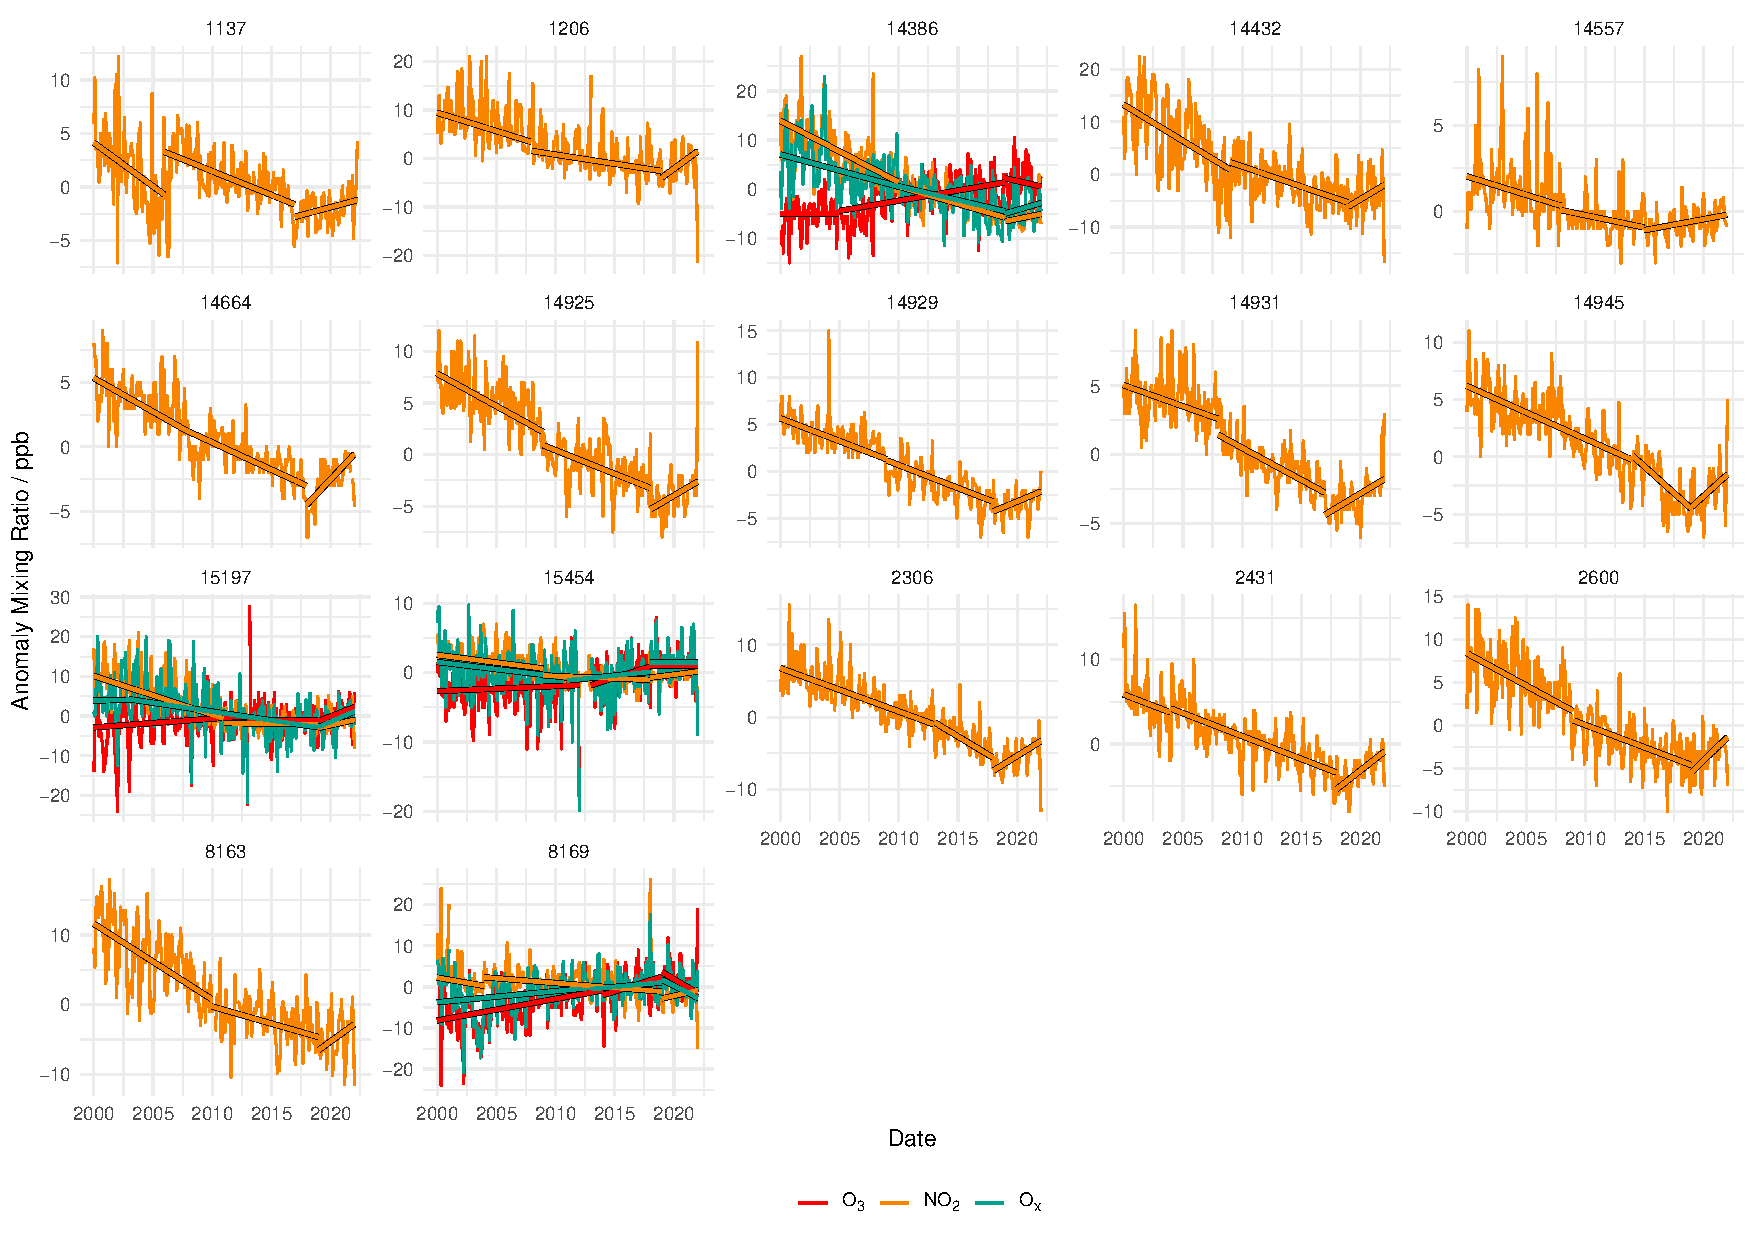
\includegraphics[height=14cm]{figures/f14_no2_in_usa.pdf}
\caption{Sites in the USA that had increasing NO\textsubscript{2} since 2015. Monthly averaged O\textsubscript{3} (red), NO\textsubscript{2} (orange) and O\textsubscript{x} (green) anomaly are shown. O\textsubscript{3} and O\textsubscript{x} trends differ from those presented elsewhere in the manuscript as the piecewise quantile regression where the second change point has been restricted to match that of the NO\textsubscript{2} at each site.}
\label{fig:no2_in_usa}
\end{sidewaysfigure}

\section{Conclusions}  %% \conclusions[modified heading if necessary]
%Trends in urban O\textsubscript{3} and NO\textsubscript{2} across the United States of America and Europe were explored between 2000 - 2021. Before exploring the trends, a broad look at the median change in mixing ratios across all sites in the USA and Europe revealed an increase in median O\textsubscript{3} mixing ratios in both Europe (+8 ppb) and the USA (+4 ppb) between 2000 and 2019. NO\textsubscript{2} median mixing ratios generally decreased over the 2000 - 2021 period, but a noticeable up-tick in NO\textsubscript{2} was observed in the USA in later years. 

Trends in urban O\textsubscript{3} and NO\textsubscript{2} were calculated from de-seasoned monitoring site data across both Europe and the USA. A quantile regression analysis was utilised to assess long-term trends, with the method extended to a piecewise approach. This allowed for some freedom to capture changes in a complex dataset, whilst being able to describe the trends with a small number of coefficients. Break points were limited to two per time series to keep the focus on long-term trends and the largest changes. One limitation to this approach is that time series with 3 or more large changes will not be well described by this method - however, after inspection of the regressions and comparison with a LOESS, two points were found to capture the structure well. The trends constructed from the piecewise regressions were evaluated by their statistical significance, and those poorly described using this methodology ranked lower in significance and were subsequently investigated less in the analysis. Piecewise segments were required to have $\ge$ 2 years of data, which limited the ability to define the most recent changes in a given time series, and such is why only Europe was analysed for the effects of the COVID-19 restrictions. 

In Europe, more sites were found to have an increasing O\textsubscript{3} trend between 2015-2021, compared to 2000-2004, with NO\textsubscript{2} trends showing the reverse effect (fewer sites increasing, and more decreasing in 2015-2021 compared to 2000- 2004). This broadly suggests that a VOC-limited relationship for O\textsubscript{3} formation could be common across urban sites in Europe. In the USA, the reverse is true, with a reduction in the number of sites with increasing O\textsubscript{3} trends in 2015-2021 compared with the 2000-2004 period, but with more sites with increasing NO\textsubscript{2} in 2015-2021 compared with 2000-2004. The majority of O\textsubscript{3} trends are positive and of high certainty (p <= 0.05) in Europe across the 20-year period. This is also broadly true for the USA, but the proportion of sites showing this trend reduces with time, alongside an increase in the number of sites with high-certainty negative trends in O\textsubscript{3} between 2010-2021. Previous studies have attributed positive urban O\textsubscript{3} trends in the USA to increasing winter O\textsubscript{3} concentrations \citep{Simon_2015}. However, differences in seasonality would not be observed in this analysis as the trends are derived from de-seasoned data. From the trends described here, the median ($\pm$ median absolute deviation) change in O\textsubscript{3} over the last two decades were calculated as 5.0 $\pm$ 4.6 ppb in Europe and 2.4 $\pm$ 4.9 ppb in the USA, with corresponding changes in NO\textsubscript{2} as -6.8 $\pm$ 3.6 and -8.4 ppb. 

Given the nature of its long lifetime and the complexity of its chemistry, when describing trends in O\textsubscript{3} it is important to look beyond the 50th percentile. A study of European ozone trends between 1995-2014 found that whilst the 50th percentile data did not show significant trends, significant trends were observed in the 5 th and 95 th percentiles ($\tau$ values) \citep{acp-18-5589-2018}. An exploration of the $\tau$ values in this study revealed smaller reductions in trend-derived change in O\textsubscript{3} mixing ratios in 2021 since 2000 for the lower $\tau$ values compared to higher values in Europe. This, coupled with the fact that generally O\textsubscript{3} trends across Europe are positive, suggests that the lowest ambient O\textsubscript{3} mixing ratios are increasing more rapidly than the highest values. This is consistent with the findings of \cite{acp-18-5589-2018}, who found that although peak O\textsubscript{3} concentrations were coming down across urban and suburban sites between 1995 - 2014 in Europe, an increase in the lower O\textsubscript{3} concentrations was observed in more than 75 \% of sites. 

An assessment of the spatio-temporal distribution of the first and second change points revealed more sites with a directional switch in O\textsubscript{3} trend across Europe were in the positive to negative direction in the first change point, but with more sites with a negative to positive second change point. In the USA dataset, the biggest switches from negative to positive in the first change point occurred in California and Florida, but a reversal of this trend from positive to negative was also observed across these states in the second change point. To supplement this, a calculation of the 4th highest daily maximum 8-hour running mean for O\textsubscript{3} (4MDA8) revealed high 4MDA8 hotspots in parts of southern Europe, but particularly in California, consistent with previous findings of \cite{fleming_2018}. Furthermore, the USA has seen significant increasing trends in NO\textsubscript{2} since 2015 at several sites. However, there are limited sites that have been used in this study with co-located NO\textsubscript{2} and O\textsubscript{3}, and the O\textsubscript{3} response is not consistent. This is not unexpected due to the wide range of conditions that an ‘urban’ site can be found in (e.g. variations in local VOC concentrations), but it should be expected that in some locations O\textsubscript{3} will be sensitive to this increase in NO\textsubscript{2}, especially if it persists.

The impact of COVID-19 on ambient mixing ratios of NO\textsubscript{2} is well studied, with one previous study estimating that NO\textsubscript{2} concentrations across urban background sites in Europe were 32 \% lower than expected in 2020 \citep{acp-21-4169-2021}. The impact of this COVID-19 effect was observed in the trend analysis of Europe described in this study, with the vast majority of directionally switching second change points in NO\textsubscript{2} occurring in 2020 in the negative to positive direction. This can be attributed to lower ambient NO\textsubscript{2} mixing ratios in 2020, leading to an increasing trend in the subsequent years as business-as-usual conditions resumed.  These increasing NO\textsubscript{2} concentrations have in some cases been accompanied by increasing O\textsubscript{3}/O\textsubscript{x} and should continue to be studied, since in many cases the prior downward trend in NO\textsubscript{2} has not resumed.


\clearpage

%% The following commands are for the statements about the availability of data sets and/or software code corresponding to the manuscript.
%% It is strongly recommended to make use of these sections in case data sets and/or software code have been part of your research the article is based on.

%\codeavailability{TEXT} %% use this section when having only software code available


%\dataavailability{TEXT} %% use this section when having only data sets available


\codedataavailability{All data for this study can be downloaded from the relevant databases. 
Code for performing the download as well as the analysis can be found at 10.5281/zenodo.14538198 \citep{drysdale_2024_14538198}} %% use this section when having data sets and software code available


%\sampleavailability{TEXT} %% use this section when having geoscientific samples available


%\videosupplement{TEXT} %% use this section when having video supplements available


%\appendix
%\section{}    %% Appendix A

%\noappendix       %% use this to mark the end of the appendix section. Otherwise the figures might be numbered incorrectly (e.g. 10 instead of 1).

%% Regarding figures and tables in appendices, the following two options are possible depending on your general handling of figures and tables in the manuscript environment:

%% Option 1: If you sorted all figures and tables into the sections of the text, please also sort the appendix figures and appendix tables into the respective appendix sections.
%% They will be correctly named automatically.

%% Option 2: If you put all figures after the reference list, please insert appendix tables and figures after the normal tables and figures.
%% To rename them correctly to A1, A2, etc., please add the following commands in front of them:

\appendixfigures  %% needs to be added in front of appendix figures

\appendixtables   %% needs to be added in front of appendix tables

%% Please add \clearpage between each table and/or figure. Further guidelines on figures and tables can be found below.



\authorcontribution{BSN and WSD equally contributed to all aspects of this manuscript's production} %% this section is mandatory

\competinginterests{The authors declare that they have no conflict of interest.} %% this section is mandatory even if you declare that no competing interests are present

\begin{acknowledgements}
The Viking cluster was used during this project, which is a high performance compute facility provided by the University of York. We are grateful for computational support from the University of York, IT Services and the Research IT team.

The Authors acknowledge Prof. James Lee for their scientific advice and Prof. David Carslaw and Dr Stuart Lacy for their advice on the statistical analysis. We also thank Dr Stuart Lacy for their help with SQL and very useful suggestions on managing large datasets. 
\end{acknowledgements}


%% REFERENCES

%% The reference list is compiled as follows:



%% Since the Copernicus LaTeX package includes the BibTeX style file copernicus.bst,
%% authors experienced with BibTeX only have to include the following two lines:
%%
 \bibliographystyle{copernicus}
 \bibliography{references}
%%
%% URLs and DOIs can be entered in your BibTeX file as:
%%
%% URL = {http://www.xyz.org/~jones/idx_g.htm}
%% DOI = {10.5194/xyz}


%% LITERATURE CITATIONS
%%
%% command                        & example result
%% \citet{jones90}|               & Jones et al. (1990)
%% \citep{jones90}|               & (Jones et al., 1990)
%% \citep{jones90,jones93}|       & (Jones et al., 1990, 1993)
%% \citep[p.~32]{jones90}|        & (Jones et al., 1990, p.~32)
%% \citep[e.g.,][]{jones90}|      & (e.g., Jones et al., 1990)
%% \citep[e.g.,][p.~32]{jones90}| & (e.g., Jones et al., 1990, p.~32)
%% \citeauthor{jones90}|          & Jones et al.
%% \citeyear{jones90}|            & 1990



%% FIGURES

%% When figures and tables are placed at the end of the MS (article in one-column style), please add \clearpage
%% between bibliography and first table and/or figure as well as between each table and/or figure.

% The figure files should be labelled correctly with Arabic numerals (e.g. fig01.jpg, fig02.png).


%% ONE-COLUMN FIGURES

%%f
%\begin{figure}[t]
%\includegraphics[width=8.3cm]{FILE NAME}
%\caption{TEXT}
%\end{figure}
%
%%% TWO-COLUMN FIGURES
%
%%f
%\begin{figure*}[t]
%\includegraphics[width=12cm]{FILE NAME}
%\caption{TEXT}
%\end{figure*}
%
%
%%% TABLES
%%%
%%% The different columns must be seperated with a & command and should
%%% end with \\ to identify the column brake.
%
%%% ONE-COLUMN TABLE
%
%%t
%\begin{table}[t]
%\caption{TEXT}
%\begin{tabular}{column = lcr}
%\tophline
%
%\middlehline
%
%\bottomhline
%\end{tabular}
%\belowtable{} % Table Footnotes
%\end{table}
%
%%% TWO-COLUMN TABLE
%
%%t
%\begin{table*}[t]
%\caption{TEXT}
%\begin{tabular}{column = lcr}
%\tophline
%
%\middlehline
%
%\bottomhline
%\end{tabular}
%\belowtable{} % Table Footnotes
%\end{table*}
%
%%% LANDSCAPE TABLE
%
%%t
%\begin{sidewaystable*}[t]
%\caption{TEXT}
%\begin{tabular}{column = lcr}
%\tophline
%
%\middlehline
%
%\bottomhline
%\end{tabular}
%\belowtable{} % Table Footnotes
%\end{sidewaystable*}
%
%
%%% MATHEMATICAL EXPRESSIONS
%
%%% All papers typeset by Copernicus Publications follow the math typesetting regulations
%%% given by the IUPAC Green Book (IUPAC: Quantities, Units and Symbols in Physical Chemistry,
%%% 2nd Edn., Blackwell Science, available at: http://old.iupac.org/publications/books/gbook/green_book_2ed.pdf, 1993).
%%%
%%% Physical quantities/variables are typeset in italic font (t for time, T for Temperature)
%%% Indices which are not defined are typeset in italic font (x, y, z, a, b, c)
%%% Items/objects which are defined are typeset in roman font (Car A, Car B)
%%% Descriptions/specifications which are defined by itself are typeset in roman font (abs, rel, ref, tot, net, ice)
%%% Abbreviations from 2 letters are typeset in roman font (RH, LAI)
%%% Vectors are identified in bold italic font using \vec{x}
%%% Matrices are identified in bold roman font
%%% Multiplication signs are typeset using the LaTeX commands \times (for vector products, grids, and exponential notations) or \cdot
%%% The character * should not be applied as mutliplication sign
%
%
%%% EQUATIONS
%
%%% Single-row equation
%
%\begin{equation}
%
%\end{equation}
%
%%% Multiline equation
%
%\begin{align}
%& 3 + 5 = 8\\
%& 3 + 5 = 8\\
%& 3 + 5 = 8
%\end{align}
%
%
%%% MATRICES
%
%\begin{matrix}
%x & y & z\\
%x & y & z\\
%x & y & z\\
%\end{matrix}
%
%
%%% ALGORITHM
%
%\begin{algorithm}
%\caption{...}
%\label{a1}
%\begin{algorithmic}
%...
%\end{algorithmic}
%\end{algorithm}
%
%
%%% CHEMICAL FORMULAS AND REACTIONS
%
%%% For formulas embedded in the text, please use \chem{}
%
%%% The reaction environment creates labels including the letter R, i.e. (R1), (R2), etc.
%
%\begin{reaction}
%%% \rightarrow should be used for normal (one-way) chemical reactions
%%% \rightleftharpoons should be used for equilibria
%%% \leftrightarrow should be used for resonance structures
%\end{reaction}
%
%
%%% PHYSICAL UNITS
%%%
%%% Please use \unit{} and apply the exponential notation


\end{document}
